%%%%%%%%%%%%%%%%%%%%%%%%%%%%%%%%%%%%%%%%%%%%%%%%%%%%%%%%%%%%%%%%%%%%%%%%%%%%%%%%
% Template for USENIX papers.
%
% History:
%
% - TEMPLATE for Usenix papers, specifically to meet requirements of
%   USENIX '05. originally a template for producing IEEE-format
%   articles using LaTeX. written by Matthew Ward, CS Department,
%   Worcester Polytechnic Institute. adapted by David Beazley for his
%   excellent SWIG paper in Proceedings, Tcl 96. turned into a
%   smartass generic template by De Clarke, with thanks to both the
%   above pioneers. Use at your own risk. Complaints to /dev/null.
%   Make it two column with no page numbering, default is 10 point.
%
% - Munged by Fred Douglis <douglis@research.att.com> 10/97 to
%   separate the .sty file from the LaTeX source template, so that
%   people can more easily include the .sty file into an existing
%   document. Also changed to more closely follow the style guidelines
%   as represented by the Word sample file.
%
% - Note that since 2010, USENIX does not require endnotes. If you
%   want foot of page notes, don't include the endnotes package in the
%   usepackage command, below.
% - This version uses the latex2e styles, not the very ancient 2.09
%   stuff.
%
% - Updated July 2018: Text block size changed from 6.5" to 7"
%
% - Updated Dec 2018 for ATC'19:
%
%   * Revised text to pass HotCRP's auto-formatting check, with
%     hotcrp.settings.submission_form.body_font_size=10pt, and
%     hotcrp.settings.submission_form.line_height=12pt
%
%   * Switched from \endnote-s to \footnote-s to match Usenix's policy.
%
%   * \section* => \begin{abstract} ... \end{abstract}
%
%   * Make template self-contained in terms of bibtex entires, to allow
%     this file to be compiled. (And changing refs style to 'plain'.)
%
%   * Make template self-contained in terms of figures, to
%     allow this file to be compiled. 
%
%   * Added packages for hyperref, embedding fonts, and improving
%     appearance.
%   
%   * Removed outdated text.
%
%%%%%%%%%%%%%%%%%%%%%%%%%%%%%%%%%%%%%%%%%%%%%%%%%%%%%%%%%%%%%%%%%%%%%%%%%%%%%%%%

\documentclass[letterpaper,twocolumn,10pt]{article}
\usepackage{usenix2019_v3}

% to be able to draw some self-contained figs
\usepackage{tikz}
\usepackage{amsmath}
\usepackage{xcolor}
\usepackage{graphicx}
\usepackage{subcaption}
\usepackage{float}
\usepackage{listings, multicol}
\usepackage{appendix}


% inlined bib file
\usepackage{filecontents}

\lstdefinelanguage{P4}{
  keywords={in, out, struct, inout, function, return, switch, exact, const, entries, enum, if, else, case, break, extern, void, bit, error, int, verify, bool, key, table, action, actions, parser, control, state, transition, select, apply, true, false},
  keywordstyle=\color{myk}\bfseries,
  keywords=[2]{boolean, string, number, objectid},
  keywordstyle=[2]\color{green}\bfseries,
  identifierstyle=\color{darkgray}\bfseries,
  sensitive=false,
  comment=[l]{//},
  morecomment=[s]{/*}{*/},
  commentstyle=\color{commentcolor}\ttfamily,
  stringstyle=\color{red}\ttfamily,
  morestring=[b]',
  morestring=[b]"
}

\lstset{
   language=P4,
%    numbers=left,
%    backgroundcolor=\color{mygray},
   extendedchars=true,
   basicstyle=\small\ttfamily\color{darkgray}\bfseries,
   showstringspaces=false,
   showspaces=false,
   tabsize=2,
   frame=single,
   breaklines=true,
   showtabs=false
}
\definecolor{mygray}{gray}{1.0}
\definecolor{commentcolor}{RGB}{0,100,0}
\definecolor{myk}{rgb}{0.0,0,0.65}

\newcommand{\hs}[1]{{\color{blue}{HS:#1}}}
\newcommand{\hse}[1]{{\color{blue}{#1}}}

% %-------------------------------------------------------------------------------
% \begin{filecontents}{\jobname.bib}
% %-------------------------------------------------------------------------------
% @Book{arpachiDusseau18:osbook,
%   author =       {Arpaci-Dusseau, Remzi H. and Arpaci-Dusseau Andrea C.},
%   title =        {Operating Systems: Three Easy Pieces},
%   publisher =    {Arpaci-Dusseau Books, LLC},
%   year =         2015,
%   edition =      {1.00},
%   note =         {\url{http://pages.cs.wisc.edu/~remzi/OSTEP/}}
% }
% @InProceedings{waldspurger02,
%   author =       {Waldspurger, Carl A.},
%   title =        {Memory resource management in {VMware ESX} server},
%   booktitle =    {USENIX Symposium on Operating System Design and
%                   Implementation (OSDI)},
%   year =         2002,
%   pages =        {181--194},
%   note =         {\url{https://www.usenix.org/legacy/event/osdi02/tech/waldspurger/waldspurger.pdf}}}
% \end{filecontents}
% 
%-------------------------------------------------------------------------------
\begin{document}
%-------------------------------------------------------------------------------

%don't want date printed
\date{}

% make title bold and 14 pt font (Latex default is non-bold, 16 pt)
\title{\Large \bf Formatting Submissions for a USENIX Conference:\\
  An (Incomplete) Example}

%for single author (just remove % characters)
\author{
{\rm Your N.\ Here}\\
Your Institution
\and
{\rm Second Name}\\
Second Institution
% copy the following lines to add more authors
% \and
% {\rm Name}\\
%Name Institution
} % end author

\maketitle

%-------------------------------------------------------------------------------
\begin{abstract}
%-------------------------------------------------------------------------------
Your abstract text goes here. Just a few facts. Whet our appetites.
Not more than 200 words, if possible, and preferably closer to 150.
\end{abstract}


\section{Introduction}

% hardware and software together, cool
Over the last decade, the synergistic development of packet-processing
hardware and software has fundamentally changed how networks are built
and operated. Hardware platforms such as
RMT~\cite{Bosshart:2013:FMF:2486001.2486011} provide tremendous
flexibility for customizing the forwarding plane without having to
fabricate new chips, while languages such as
P4~\cite{Bosshart:2014:PPP:2656877.2656890, p4lang} enable programmers
to describe rich packet-processing functions in terms of high-level
abstractions such as parsers and match-action tables.

In order to support different kinds of targets (e.g., software
switches, ASICs, FPGAs, etc.), P4 allows programmable and
fixed-function blocks to be arranged into different layouts as
specified by an architecture declaration. For example, the Protocol
Independent Switch Architecture
(PISA)~\cite{Bosshart:2013:FMF:2486001.2486011} models a switch with a
programmable parser, programmable ingress pipeline, fixed-function
scheduler and queues, programmable egress pipeline, and programmable
deparser. PISA programs supply P4 code for each programmable block.
But while this design allows the language to flexibly accommodate a
wide range of targets, it also creates a tight coupling between
programs and architectures, which makes it difficult to write programs
in a compositional manner or reuse common code fragments in different
programs.

\hse{TODO: }

For example, \texttt{switch.p4}~\cite{switch.p4} handles several dozen
different protocols and functions (e.g., L2 switching, L3 routing,
tunneling, etc.,). But the code is written against a global collection
of metadata and parsed headers. To use the code in 
\texttt{switch.p4} to implement an Ethernet switch, it would be
necessary to detangle the L2-specific functionality from the
extraneous code in the rest of the program. Without a detailed
understanding of the overall structure of the top-level program, it is
difficult or impossible to reuse code fragments at finer granularity.

% \section{Use Case}
% Consider a simple scenario with two code fragments, as shown in Figure~\ref{fig:ipv4.p4.l2.p4}.

The first code fragment, \texttt{ipv4.p4}, parses the IPv4 header, uses
longest-prefix matching to determine the next hop, decrements the
\texttt{ttl} field and, finally, deparses the packet. The second
snippet, \texttt{l2.p4}, parses the Ethernet header, and modifies the
ethernet addresses using the next hop, which is supplied as an
argument, and finally deparses the packet. Note that neither
\texttt{ipv4.p4} nor \texttt{l2.p4} is a complete packet-processing
program: the former does not generate a functionally correct packets,
while the latter is parameterized on the next hop and so does not
specify forwarding behavior. However, we could combine \texttt{l2.p4}
with any other routing scheme (e.g., IPv6, MPLS, etc.) to obtain a
valid program. 

% \begin{figure*}[!ht]
% \noindent \begin{minipage}[t]{.48\textwidth}
% \begin{lstlisting}[frame=none]
% // ipv4.p4
% struct meta_t { bit<16> type; }
% parser P(packet_in pin, out hdr_t ph, inout meta_t m) {
%   state start {
%     transition select(m.type) {
%       0x0800: parse_ipv4; 
%     }
%   }
%   state parse_ipv4 { 
%     pin.extract(ph.ipv4); 
%     transition accept; 
%   }
% }
% control Pipe(inout hdr_t ph, out bit<16> nexthop_id, inout sm_t sm) {
%   action process(bit<16> nh) {
%     ph.ipv4.ttl = ph.ipv4 - 1;
%     nexthop_id = nh;// setting out param
%   }
%   table ipv4_lpm_tbl {
%     key = { ph.ipv4.dstAddr : lpm } 
%     actions = { process; }
%   }
%   apply { ipv4_lpm_tbl.apply(); }
% }
% \end{lstlisting}
% \end{minipage}\vline
% \hfill\begin{minipage}[t]{.48\textwidth}
% \begin{lstlisting}[frame=none]
% control D(packet_out po, in hdr_t ph) {
%   apply { po.emit(ph.ipv4); }
% }
% // l2.p4
% parser P(packet_in pin, out hdr_t ph) {
%   state start { pin.extract(ph.eth); }
% }
% control Pipe(inout hdr_t ph, inout sm_t sm, 
%              in bit<16> nexthop_id) {
%   action drop () {}           
%   action forward(bit<48> dest_mac, bit<48> src_mac, bit<8> port) {
%     ph.eth.dstMac = dest_mac;
%     ph.eth.srcMac = src_mac;
%     sm.out_port = port;    
%   }
%   table forward_tbl {
%     key = { nexthop_id : exact; } 
%     actions = { process; drop; }
%   }
%   apply {
%     forward_tbl.apply(); 
%   }
% }
% control D(packet_out po, in hdr_t ph) {
%   apply { po.emit(ph.eth); }
% }
% \end{lstlisting}
% \end{minipage}
% % \vspace*{-10pt}
% \caption{Example: \texttt{ipv4.p4} and \texttt{l2.p4}.}
% \label{fig:ipv4.p4.l2.p4}
% \end{figure*}


%% The current ecosystem of programmable data plane enforces programmers
%% to write code amenable to the target device's data plane architecture
%% and pipeline. Programmers write code for programmable blocks taking
%% into account their location in pipeline rather than compilers
%% automatically allocating code to the appropriate blocks. We believe
%% that devices should only expose abstraction for processing blocks and
%% the onus of code allocation to the blocks in pipeline should be on
%% compilers for the devices.

There is some prior work on modular composition of P4 programs.
Systems such as HyPer4 \cite{Hancock:2016:HUP:2999572.2999607},
HyperV~\cite{8038396}, and
P4Visor~\cite{Zheng:2018:PLV:3281411.3281436} provide constructs for
merging independent programs onto a single device. However, these
systems only handle programs that describe end-to-end
packet-processing functions. Hence, they lack mechanisms for enabling
selective reuse of library code, specifying interfaces between
modules, and facilitating inter-module communication. To write truly
modular P4 programs, a fundamentally different approach is needed.

To this end, this paper presents the design and (prototype)
implementation of $\mu$P4, a new architecture that provides
fine-grained abstractions for constructing data plane programs.
$\mu$P4 consists of two components, Micro Switch Architecture
($\mu$SA), which distills packet processing to its essence, and
abstracts away from device-specific structure, and a compiler,
$\mu$P4C, that maps one or more $\mu$SA programs to a standard PISA
pipeline. 

This paper makes the following contributions.
\begin{itemize}
\item We motivate the need for modular data plane programming using a
  series of realistic examples.
\item We introduce $\mu$ SA, a new P4 architecture designed to enable
  fine-grained composition of program snippets.
\item We develop techniques for compiling $\mu$SA programs to the
  standard PISA model, including merging programs composed together 
  \hse{and scheduling them onto a single PISA pipeline}.
%   including merging programs composed together in
%   parallel or in sequence onto a single PISA pipeline.
\end{itemize}

Although much work remains, we believe that $\mu$ SA represents a
promising first step toward enabling modular data plane programs.


\section{Examples}

\hse{TODO:  SRv6, routing, ingress-egress NAT}
% \subsection*{Compiling $\mu$P4 Programs}
% $\mu$P4C provides well-known mechanism, compile and link, to generate executable code.
% If a program does not contain a package instance named main, $\mu$P4C generates a library by compiling it to an Intermediate Representation (IR) in json format (Figure \ref{fig:compiling-msa-programs}).
% It also generates architecture-independent control-plane APIs, P4Runtime \cite{p4runtime} files.
% % $\mu$P4C's front-end generates P4Runtime files containing only APIs for match-action tables in the program.
% % The front-end of $\mu$P4C resolves used-package types with their declarations or definitions.
% \begin{figure}
%     \centering
%     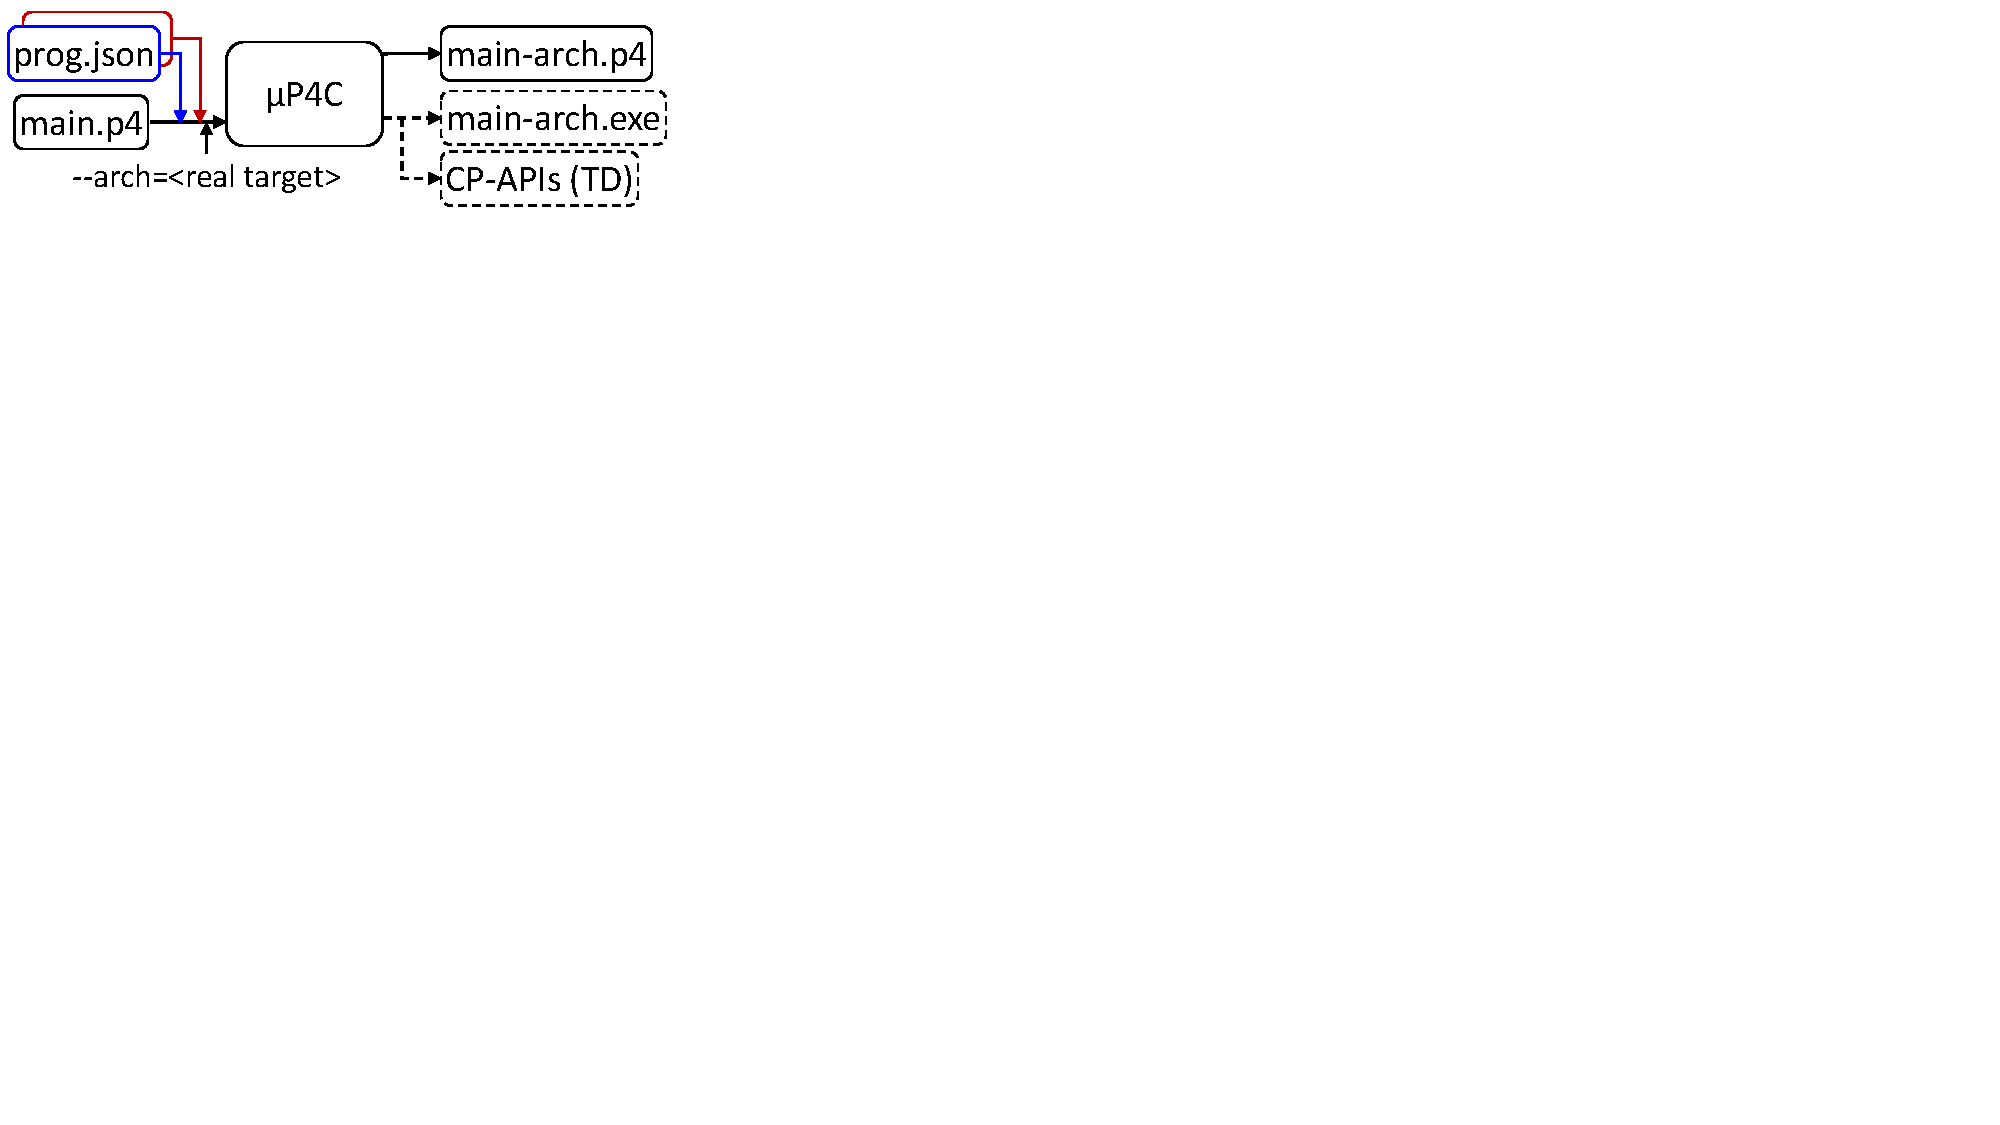
\includegraphics[trim=2 400 565 2, clip,scale=0.5]{mp4c-compiler}
%     \caption{Compiling $\mu$SA programs}
% \label{fig:compiling-msa-programs}
% \end{figure}
% Programmers can include files containing definitions of types (e.g., struct types of in and out parameters) used in runtime interfaces of packages in libraries.
% $\mu$P4C compiler generates either source P4 code for the specified architecture or executable with architecture-specific CP APIs.


\section{Micro Switch Architecture}
\label{section:micro-switch-architecture}
$\mu$P4 is designed to provides logical abstraction for data plane pipelines to enable code reuse across different real target devices without compromising expressiveness and packet-processing features.
We consider $\mu$P4 as a logical target device with an abstract packet-processing model.
We model every $\mu$P4-program as a black-box, micro-switch, that processes packet byte-stream, intrinsic metadata and arguments for user-defined parameters.
The black-box model hides implementation details (headers types, user-defined metadata, programmable blocks etc.,) of the programs.
$\mu$P4 executes programs using the packet-processing model shown in Figure \ref{fig:mp4-packet-processing-model}.
\begin{figure}
    \centering
    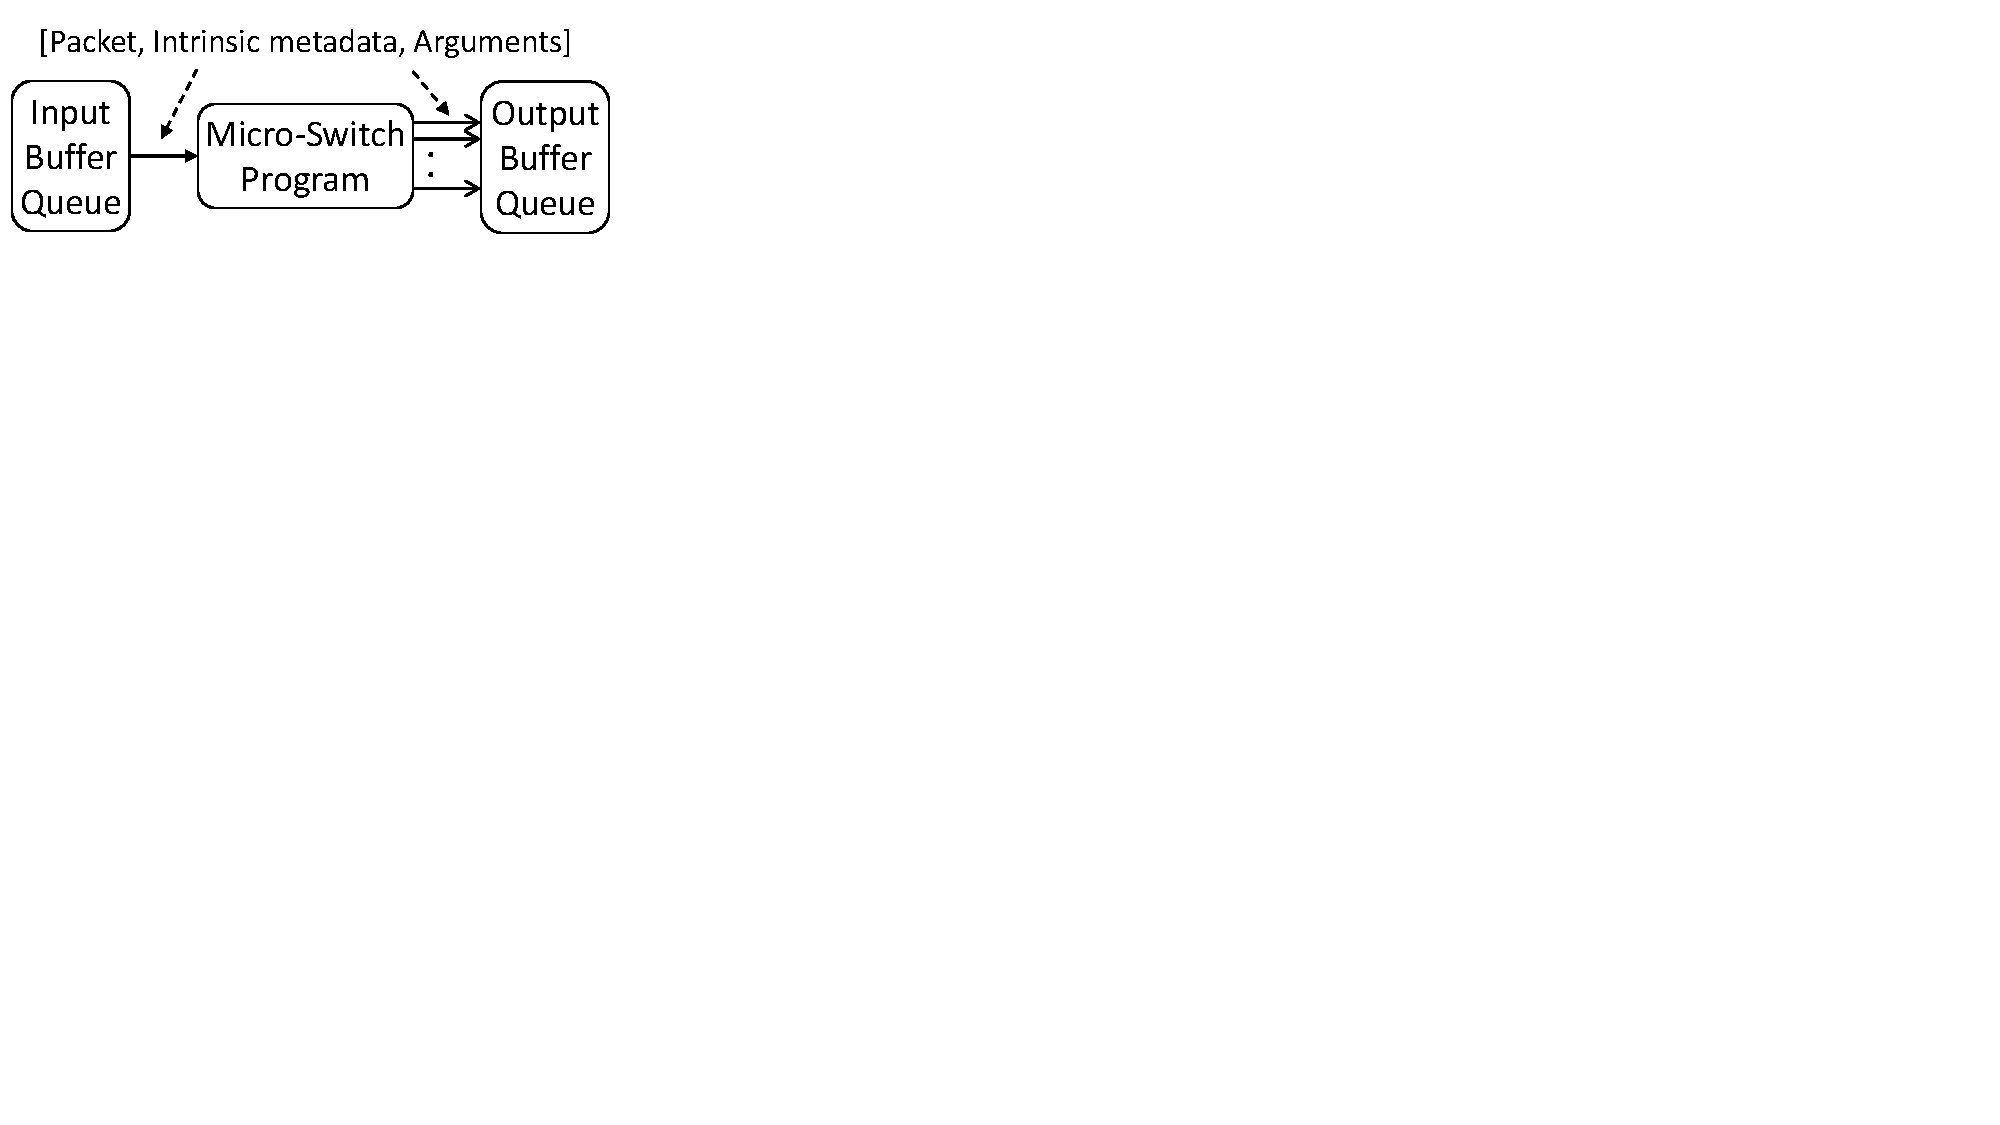
\includegraphics[trim=0 420 667 0, clip, scale=0.5]{microp4-program-model}
    \caption{Packet-Processing model of $\mu$P4 programs}
    \label{fig:mp4-packet-processing-model}
\end{figure}
$\mu$P4 fetches an element form a logical input buffer queue, executes the program and writes one or more elements to a logical output buffer queue.
Every element of the buffers comprises a packet bit-stream, intrinsic metadata (e.g., ingress\_port, egress\_port, packet\_length etc., ) and input arguments or output arguments associated with the packet.
Using this notion of program execution, we define program interfaces and packet-processing pipelines for $\mu$P4 as a port of its data plane architecture, $\mu$SA.
In addition, $\mu$SA defines a set of logical externs providing various packet-processing constructs available in fixed-function blocks (e.g., packet duplication) of real-target devices' pipelines.


\subsection{Pipelines and Interfaces}
\label{subsection:pipelines}
$\mu$SA has two types logical pipeline, Micro and Orchestration, shown in Figure \ref{fig:msa-pipelines}
% $\mu$SA's logical externs can be instantiated and used within control blocks of the $\mu$SA pipelines.
Micro pipeline comprises of a Parser, a Micro control and a Deparser block.
$\mu$SA does not allow conditional statements in deparser blocks of its pipelines.
For each pipeline type, it exposes one or more interface types.
Each interface type comprises of a set of declarations for programmable blocks and runtime signature.
\begin{figure}
    \centering
    \begin{subfigure}{0.59\linewidth}
        \centering
        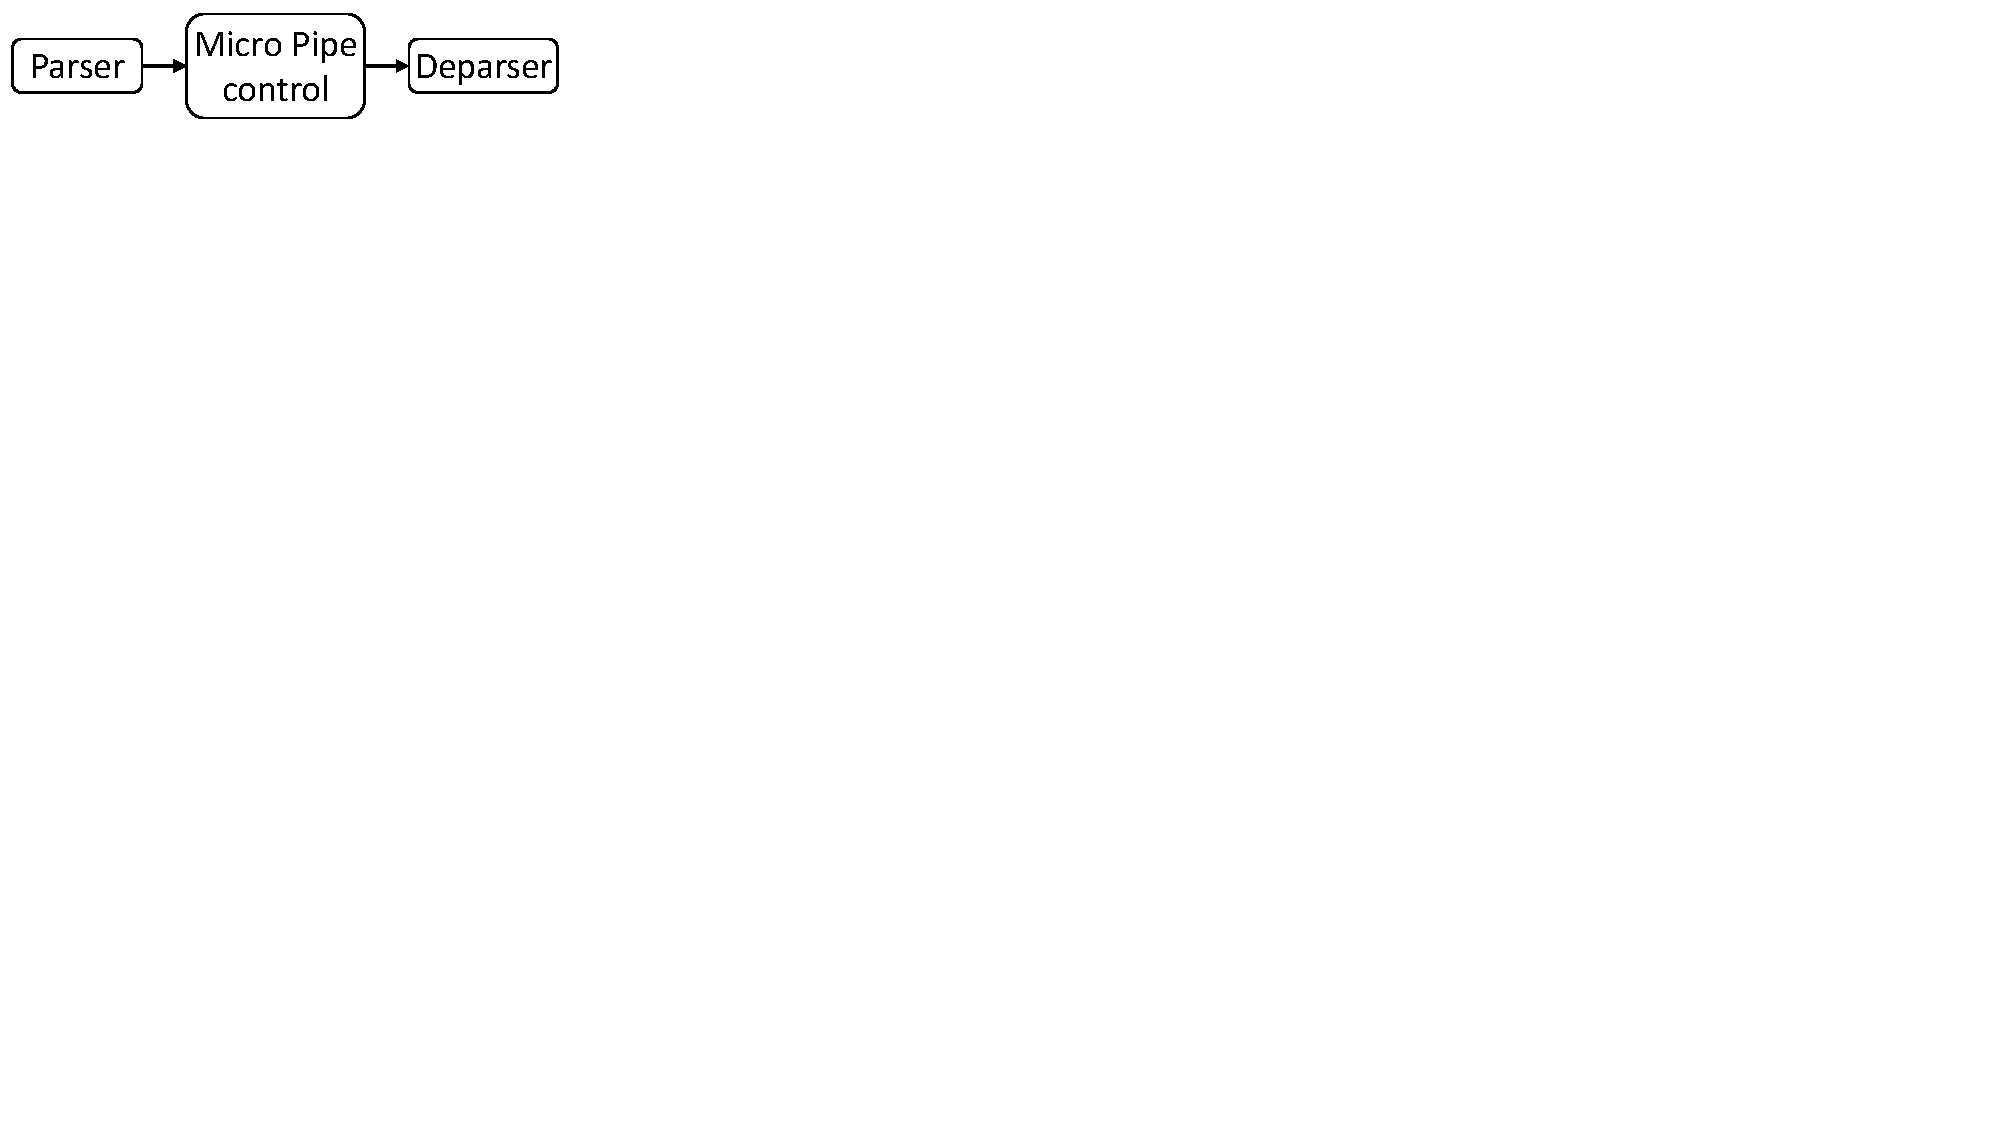
\includegraphics[trim=0 482 692 0, clip,scale=0.45]{msa-pipeline}
        \caption{Micro}
%         \label{subfig:micro}
    \end{subfigure}\vline
    \begin{subfigure}{0.41\linewidth}
        \centering
        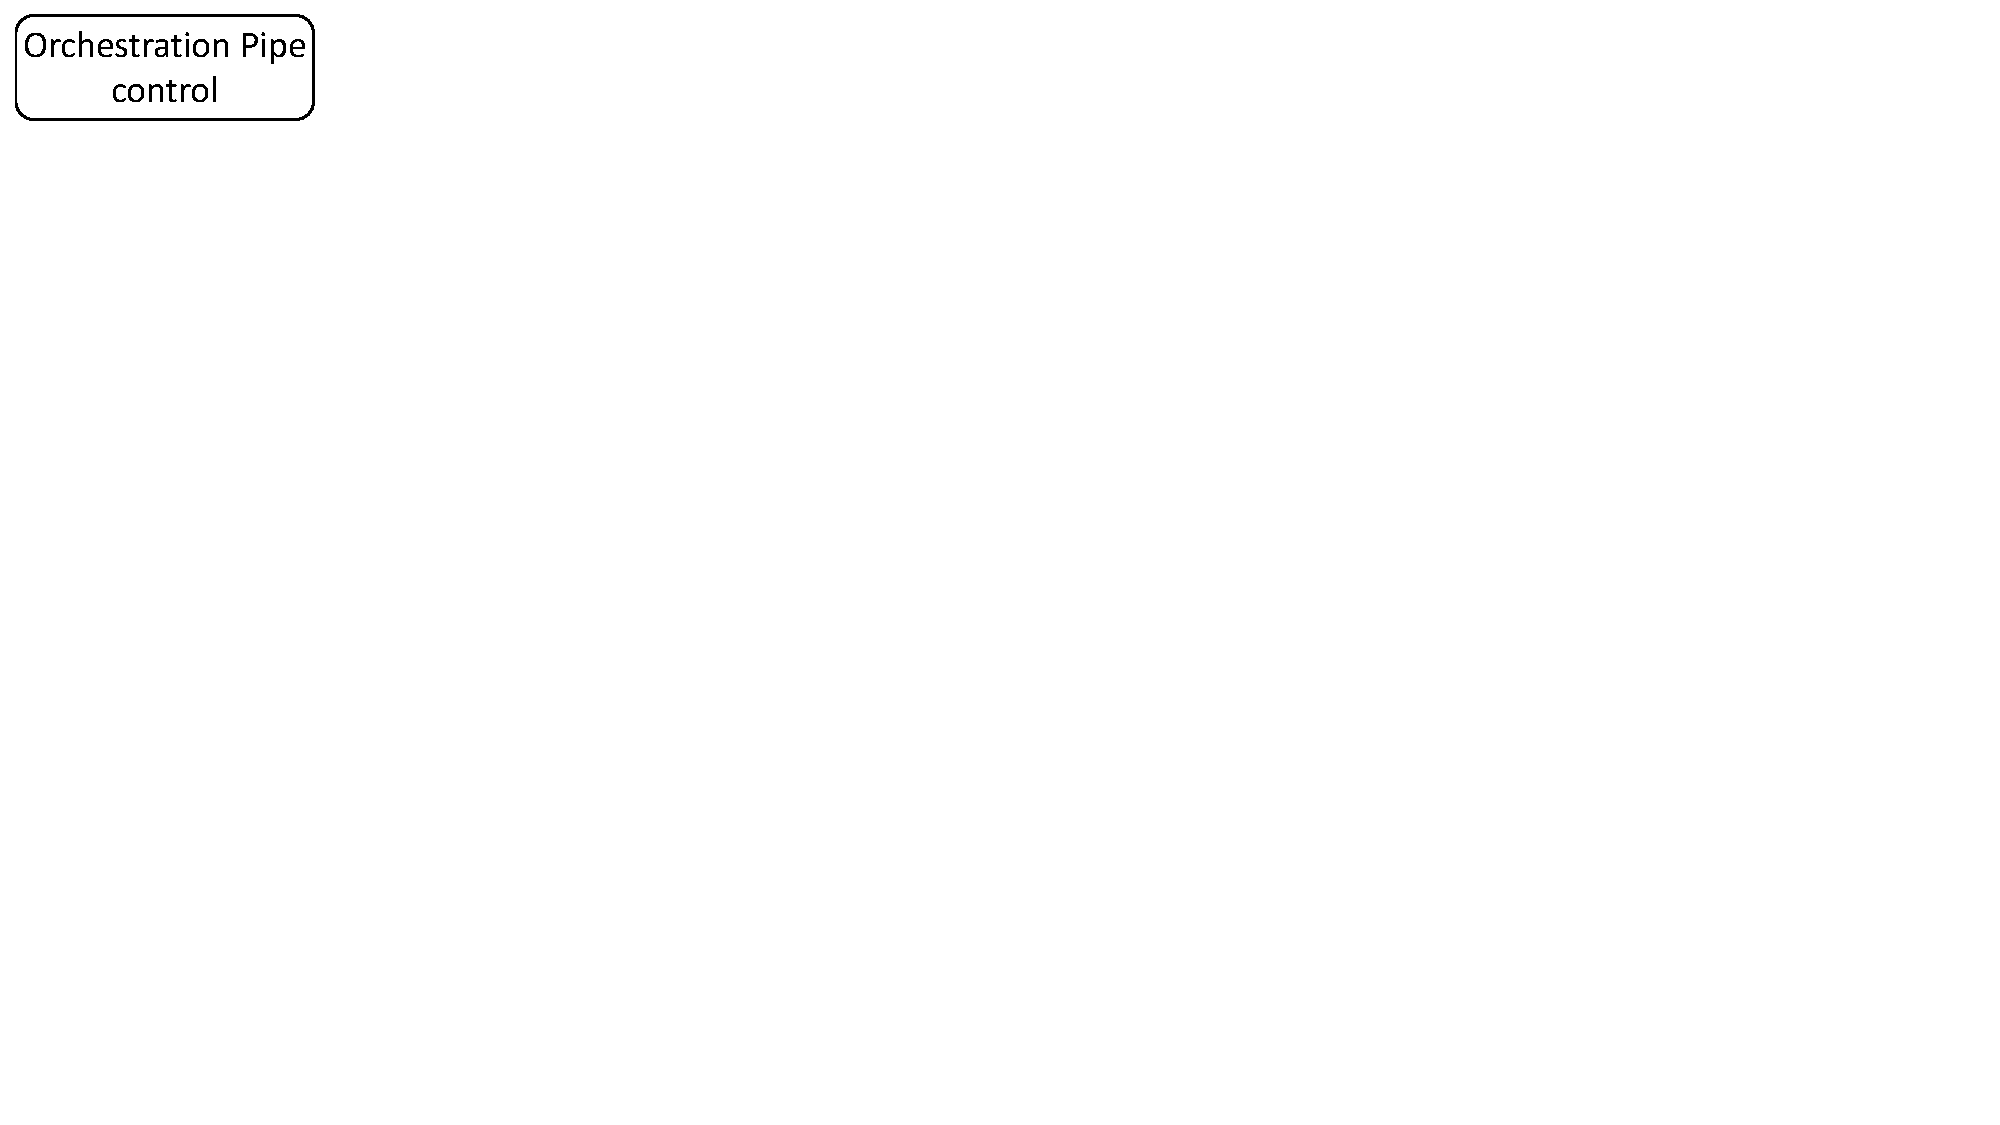
\includegraphics[trim=0 480 805 0,clip,scale=0.45]{micro-orchestration-pipeline}
        \caption{Orchestration}
%         \label{subfig:orchestration}
    \end{subfigure}
\caption{$\mu$SA Pipelines}
\label{fig:msa-pipelines}
\end{figure}
Programmers can provide implementations of the interface types to create user-defined P4 package types.
To implement an interface type, programmers need to implement all the programmable blocks of the interface type.
Programmers can instantiate variable of user-defined package types and invoke the instances using \texttt{apply} built-in method similar to control blocks.
Every incoming packet is parsed and validated by the parser, if parser terminates in \texttt{accept} state, then execution-control is transferred to micro control block.
If the execution-control reaches till the end of the micro control block, packet is processed by the deparser block.
Orchestration pipeline has only a control block, named orchestration.

$\mu$SA declares thress interface types, Unicast, Multicast and Orchestration.
\begin{lstlisting}[frame=none]
Unicast<H,M,I,O,IO>
  (pkt p, inout sm_t sm, es_t es, in I i_param, out O o_param, inout IO io_param) // Runtime Params
  (Par<H,M,I,O> p, Con<H,M,I,O,IO> c, Dep<H> d); // Programmable Blocks
Multicast<H,M,I,O>
  (pkt p, in sm_t sm, es_t es, in I i_param, out_buf<O> ob)
  (Par<H,M,I> p, Con<H,M,I,O> c, Dep<H> d); 
Orchestration<I,O>
  (in_buf<I> ib, out_buf<O> ob)
  (Con<I,O> c);
\end{lstlisting}
Programmers can implement programmable blocks declared for Micro pipeline to create custom package types having runtime signature same as unicast or multicast interface.
Similarly, Orchestration interface is associated with Orchestration pipeline.
The \texttt{pkt} is an extern type representing packet. 
The \texttt{sm\_t} is struct type containing intrinsic metadata (e.g., pkt\_in\_port, pkt\_length etc.,).
The \texttt{es\_t} extern represent intrinsic metadata related to output port of the packet in the pipeline along with queuing related metadata.
\texttt{in\_buf} and \texttt{out\_buf} externs represent logical input and output buffer of $\mu$P4 packet-processing model (Figure \ref{fig:mp4-packet-processing-model})
Next, we give overview of logical externs defined in $\mu$SA along with their example usage.

% It defines standard intrinsic metadata as \emph{sm\_t} as a struct type.
% The fields of this struct provide basic information populated by the target e.g., \emph{packet\_length}.

% Some fields are not mutable, however $\mu$SA allows to declare instances of the struct and perform assignment operation between two instances to create copies.

\subsection{Logical Externs}
\label{subsection:logical-externs}
\subsubsection{Packet Extern}
$\mu$P4 does not make use of packet extern defined in P4 core library.
Instead, it models packets using an extern object, \texttt{pkt}, declared in $\mu$SA.
% as shown in Figure \ref{fig:pkt-externs}.
The \texttt{pkt} extern can be instantiated only inside the control block of the orchestration pipeline.
$\mu$P4 mandates to initialize programmer-declared \texttt{pkt} instances in the control block using other instances.
The \texttt{pkt} extern object contains \texttt{copy\_from} having a parameter of its own type as shown in code snippet below.
\begin{lstlisting}[frame=none]
extern pkt {
  void copy_from(pkt pkt_arg_inst);
}
\end{lstlisting}
The \texttt{copy\_from} method initializes its calling instance with content of \texttt{pkt\_arg\_inst} without modifying it.
$\mu$SA provides two externs objects, \texttt{extractor} and \texttt{emitter}, to facilitate data extraction from and insertion into packets.
The \texttt{extractor} and \texttt{emitter} externs can not be instantiated, their instances are provided by the architecture as parameters in parser and deparser declarations of Micro pipeline programmable blocks. 


\subsubsection{Correlated Intrinsic Metadata}
$\mu$P4 maintains logical intrinsic metadata. 
For every real target device, $\mu$P4C maintains mapping of its logical intrinsic metadata with the metadata of real target.
Many intrinsic per-packet metadata provided by architectures of real target devices are correlated.
For example, many real target devices allow to measure every packet's queuing latency through the device.
The timestamps required to compute queuing latency can be measured only after the packet's out port is finalized and packet is enqueued in appropriate queue.
$\mu$SA models correlated intrinsic metadata using stateful logical externs.
$\mu$SA captures dependency among correlated intrinsic metadata using stateful extern objects.
$\mu$SA declares \texttt{es\_t} extern object with methods to access 
The \texttt{es\_t} extern object contains methods to manipulate and access interdependent intrinsic metadata.
For example, \texttt{set\_out\_port} and \texttt{get\_out\_port} allows to set and get output port for the packet.
In addition, $\mu$SA declares an enumerator, called \texttt{meta\_t}.
Each value in the enumerator associated with a immutable intrinsic metadata populated by only target for every packet (e.g., \texttt{IN\_TIMESTAMP}, \texttt{OUT\_TIMESTAMP} etc).
The \texttt{es\_t} extern declares a two-parameters method, \texttt{get\_value}, that allows to read values populated by the target.
The first parameter with \texttt{in} direction is of \texttt{meta\_t} type indicating a particular metadata field.
The second parameter with \texttt{out} direction provides value of the field.

% $\mu$P4C allows repeated usage of the extern's functions in the single control block of $\mu$SA pipelines.
% If \emph{get\_value} occurs before \emph{set\_egress\_port} on any possible execution-control path, $\mu$P4C raises a compile-time error.
\begin{figure*}
\noindent \begin{minipage}[t]{.50\textwidth}
\begin{lstlisting}[frame=none]
// ipv6.p4
header ipv6_h { ... }; 
struct ipv6_ht { ipv6_h ip };
parser P(extractor ex, pkt p, out ipv6_ht h) {
  state start {
    ex.extract(p, h.ip); transition accept;
  }
}
control C(pkt p, inout ipv6_ht h, inout sm_t sm, es_t es, out bit<16> nexthop) {
  action process(bit<16> nh) {
    h.ip.hopLimit = h.ip.hopLimit - 1;
    nexthop = nh;// setting out param
  }
  table ipv6_lpm_tbl {
    key = { h.ip.dstAddr : lpm } 
    actions = { process; }
  }
  apply { ipv6_lpm_tbl.apply(); }
}
control D(emitter em, pkt p, in ipv6_ht h) {
  apply { em.emit(p, h.ip); }
}
// router.p4
// runtime interfaces of callee programs
ipv6(pkt p, inout sm_t sm, es_t es, out bit<16> nexthop);
ipv4(pkt p, inout sm_t sm, es_t es, out bit<16> nexthop);
mpls(pkt p, inout sm_t sm, es_t es);
\end{lstlisting}
\end{minipage}\hspace{-4pt}\vline
\hfill\begin{minipage}[t]{.50\textwidth}
\begin{lstlisting}[frame=none]
parser P(extractor ex, pkt p, out hdr_t h) {
  state start {
    ex.extract(p, h.eth); transition accept;
  }
}
control C(pkt p, inout hdr_t h, inout sm_t sm, es_t es) {
  bit<16> nh_id;
  ipv4() ipv4_i; ipv6() ipv6_i; mpls() mpls_i;
  action drop () {}           
  action forward(bit<48> dmac, bit<48> smac, bit<8> port) {
    h.eth.dstMac = dmac; h.eth.srcMac = smac;
    es.set_out_port(port);
  }
  table forward_tbl {
    key = { nh_id : exact; } 
    actions = { forward; drop; }
  }
  apply {
    switch (h.eth.etherType) {
      0x0800 : ipv4_i.apply(p, sm, es, nh_id);
      0x86DD : ipv6_i.apply(p, sm, es, nh_id);
      0x8847 : mpls_i.apply(p, sm, es);
    }
    forward_tbl.apply(); 
  }
}
control D(emitter em, pkt p, in hdr_t h) {
  apply { em.emit(p, h.eth); }
}
\end{lstlisting}
\end{minipage}
\caption{Modular Router using $\mu$ SA}
\label{fig:modular-router}
\end{figure*}

\begin{figure}
\begin{subfigure}[b]{\linewidth}
 \begin{lstlisting}[frame=none]
// srv6.p4
header ext_routing_h { ... }; 
header srh_h { ... }; header ipv6_h { ... }; 
struct srv_ht { 
  ipv6_h ipv6; ext_routing_h er; srh_h sr;
};
parser P(extractor e, pkt p, out srv_ht h) {
  state start {
    e.extract(p, h.ipv6);
    transition select (h.ipv6.nextHdr) {
      0x2B : parse_routing_hdr; }
  }
  state parse_routing_hdr { ... }
  state parse_srh { ... }
}
control C(pkt p, inout srv_ht h, inout sm_t sm, es_t es) {
  apply { // copy appropriate segment address from h.sr to h.ipv6.destAddr}
}
control D(emitter em, pkt p, in srv_ht h) {
  apply { 
    em.emit(p, h.ipv6);
    em.emit(p, h.er); em.emit(p, h.sr);
  }
}
\end{lstlisting}
\caption{Source Routing Header Processing}
\end{subfigure}
\begin{subfigure}[b]{\linewidth}
 \begin{lstlisting}[frame=none]
apply {
  switch (h.eth.etherType) {
    0x86DD :  { 
      srv6_i.apply(p, sm, es);
      ipv6_i.apply(p, sm, es, nh_id);
    }
  }
  forward_tbl.apply(); 
}
\end{lstlisting}
\caption{Extending Modular Router}
\end{subfigure}
\label{fig:multi-packe}
\caption{Incremental Development}
\end{figure}


\begin{figure}
\begin{lstlisting}[frame=none]
struct out_t { /* empty */ }
control mc(pkt p, hdr_t h, sm_t s, es_t e, mc_buf<hdr_t, out_t> hb) {
  mc_engine mce;  PktInstId_t id; 
  out_t  oa;
  action replicate(GroupId_t gid) {
    mce.set_mc_group(gid);
  }
  table MulticastRouting{
    key = { h.ipv4.dstAddr : exact; } 
    actions = { replicate; }
  }
  table mac{
    key = { es.get_port() : exact; } 
    actions = { mac_update; }
  }
  apply {
    MulticastRouting.apply();
    mce.apply(es, id);//similar to fork in C
    mac.apply();
    hb.enqueue(h, sm, es, oa);
  }
}
\end{lstlisting}
\caption{Multicast Execution}
\label{fig:multicast-execution}
\end{figure}

% \begin{figure}
% \begin{lstlisting}[frame=none]
% // interface for traffic mirror function
% mirror(pkt, inout sm_t, es_t);
% router(pkt, inout sm_t, es_t);
% struct e_t {};
% control rm(pkt p, inout sm_t sm, es_t es, out_buf<e_t> ob) {
%   pkt pm;  es_t es_m;  sm_t sm, sm_m;
%   apply {
%     pm.copy_from(p); sm_m = sm; 
%     es_m.copy_from(es)
%     router.apply(p, sm, es);
%     mirror.apply(pm, sm_m, es_m);
%     // stores the results in out_buf
%     ob.enqueue(p, sm, es);
%     ob.enqueue(pm, sm_m, es_m);
%   }
% }
% \end{lstlisting}
% \caption{Multi-Packet Processing}
% \label{fig:multi-packet-processing}
% \end{figure}


\begin{figure}
 \begin{lstlisting}[frame=none]
struct e_t {};  struct h_t { ... };
prog(pkt, inout sm_t, es_t, out h_t);
test(pkt, inout sm_t, es_t, out h_t);
log(pkt, inout sm_t, es_t, in h_t, in h_t);
control validate(pkt p, inout sm_t sm, es_t es, out_buf<e_t> ob) {
        pkt pt, pm;  es_t est, esm;  
        sm_t smt, smm; h_t hp, ht;
slice#  apply {
  1  c1   pm.copy_from(p); smm = sm; 
  1       esm.copy_from(es);
  3  c3   pt.copy_from(p); smt = sm; 
  3       est.copy_from(es);
 2,1      prog.apply(p, sm, es, hp); 
 3,1      test.apply(pt, smt, est, ht); 
  1       if (hp != ht) {
  1         log.apply(pm, smm, esm, hp, ht);
  1         ob.enqueue(pm, smm, esm);
  1       }
  3       smt.drop = true;
  2       ob.enqueue(p, sm, es);
  3       ob.enqueue(pt, smt, est);
        }
     }
\end{lstlisting}
\caption{Multi-Packet Processing}
\label{fig:multi-packet-processing}
\end{figure}


% \subsubsection{Multicast Extern}
% $\mu$SA's multicast extern (Figure \ref{fig:msa-multicast-extern}) can be instantiated in the control blocks of its pipelines.
% The \emph{set\_multicast\_group} can be used to assign replication group to the packet. 
% The \emph{apply} function is allowed to use only in \emph{apply} body control blocks. 
% It is analogous to \emph{fork} system call in C except that processing of original packet terminates at the apply call.
% It returns instance id of the replica and populates the es\_t instance with the port id set by the control plane.
% $\mu$P4C translates this extern to multicast mechanism defined in architectures of real targets.
% We assume these architectures would have sufficient fields to program their replication engine, so that a combination of the fields can be used as packet instance id.


% \begin{figure}[H]
% \begin{lstlisting}
% struct out_t { bit<16> data;}
% control mc(pkt_in pi, sm_t sm, es_t es, 
%         hs_t h, ia_t ia, mc_buf<hs_t, out_t> hb) {
%   mc_engine mce;  pkt_inst_id_t id; 
%   out_t  oa;
%   table t{
%     key = {} actions = { mce.set_mc_group; drop; }
%   }
%   table mac{
%     key = { es.get_port(); } 
%     actions = { mac_update; }
%   }
%   apply {
%     id = mce.apply(es); // equivalent to fork in C
%     mac.apply();
%     hb.enqueue(h, sm, es, oa);
%   }
% }
% control dep(pkt_out<o_a> ob, 
%             mc_buf<hs_t, out_arg_t> hb) {
%   hs_t ph; out_arg_t oa; pkt_out po;
%   hb.dequeue(ph, sm, es, oa);
%   // deparser code 
%   ob.enqueue(po, sm, es, oa);
% }
% \end{lstlisting}
% \caption{Multicast Execution}
% \label{fig:multicast-execution}
% \end{figure}







\section{Compiler}
$\mu$P4C transforms parsers and deparsers of the main and callee programs into match-action control blocks.
It synthesizes new parser and deparser for the main program.
The synthesized parser accepts every packet with length greater than the minimum length, called \emph{min-packet-size}, derived by static-analysis of the program.
For every accepted packet, the synthesized parser at most extracts a fixed number, called \emph{extract-length}, of bytes to a stack, called \emph{byte-stack}, of one-byte headers.
Programs may increase or decrease size of packets, therefore, the size of byte-stack can be greater than extract-length.
The synthesized deparser emits all valid one-byte headers from the byte-stack.




We perform compile-time analysis of parser, control and deparser blocks to estimate min-packet-size, extract-length and the size of byte-stack to process packets, as explained in section \ref{subsection:extract-length-and-byte-stack-size}. 
$\mu$P4C treats byte-stack as a packet and executes transformed parsers and deparsers in the match-action stages of the target's pipeline.
For each program, $\mu$P4C creates metadata variables, called \texttt{field-variables} for the header fields used in the program's control block.
The header fields are substituted with the metadata variables in control blocks of the program.
$\mu$P4C discards types and instances of the headers of each program.
$\mu$P4C synthesizes a single bit \emph{valid} metadata variable for each header instance to record its presence in the packet.
\texttt{setValid} and \texttt{setInvalid} method-call statements of every header instance is replaced with assignments on the related \emph{valid} metadata variable.
Execution of parsers in match-action stages copy values from the appropriate locations in the byte-stack to the variables.
It also updates valid metadata variables which are later used by the deparser to copy back field-variables to byte-stack.


\hs{TODO: define Simple parser as a parser without stacks and variable-length header. \ref{subsection:parser-to-match-action-table} discuss about converting simple parser into a match-action table. section \ref{subsection:header-stacks-variable-length-headers} converts parsers with header stacks or variable-length header into simple parser}


\subsection{Extract Length and Byte-Stack Size}
\label{subsection:extract-length-and-byte-stack-size}
The symbolic execution recursively evaluates extract-length and byte-stack size of every callee program in every control path in the CFG of the caller's control block.
The symbolic execution of a parser block enumerates every possible path from the start to the accept state in the parse graph.
For every path, it computes total number of bytes extracted by \texttt{extract} method call statements.
The \texttt{extract} method call statements on a path are evaluated by increasing the number of extracted bytes by size of the header instance specified in the argument.
We define the length of a path $x$ in the parse graph a program $a$'s parser, $lp_{a}(x)$, as total number of bytes extracted from the start to the accept state.
And, the extract-length of a program $a$'s parser is defined as the longest path in its parse graph, as shown in (\ref{extract-length-parser}).
Programs' extract-lengths also depend on the callees in their control blocks.
For a program $a$'s control block, we define the extract-length, $lc_{a}(x)$, of a control path $x$ in the CFG of the control block as the maximum number of bytes required to process all the callees in the path.
The extract-length of the program $a$'s control block is defined as longest path in the CFG (\ref{extract-length-control}).
A program $a$'s extract-length, $\mathcal{E}l(a)$, is sum of extract-lengths of its parser and control block.
It is necessary to discuss increase and decrease in packet size, before we explain our approach to estimate extract-length of a control path ($lc_{a}(x)$) and byte-stack size for a program.
\begin{align}
E_{p}(a)\; =& \; \max_{x}\left\{lp_{a}(x)\right\} \label{extract-length-parser} \\
E_{c}(a)\; =& \; \max_{x}\left\{lc_{a}(x)\right\} \label{extract-length-control} \\
\mathcal{E}l(a)\; =& \; E_{p}(a) + E_{c}(a) \label{extract-length-program}
\end{align}



To estimate maximum decrease, we consider that a packet contains all the header instances that are set to valid or invalid on the control path.
For maximum increase, we consider that a packet does not contain any header instance that is set to valid or invalid on the control path. 
We evaluate header instances' \texttt{setValid} and \texttt{setInvalid} method call statements on every path in the CFG of the control block.
We denote increase and decrease in packet size on a path $x$ in the CFG of control block of a program $a$ using $i_{a}(x)$ and $d_{a}(x)$, respectively.
Similarly, $\Delta(a)$ and $\delta(a)$ denote maximum increase and decrease in packet size by a program $a$.
$i_{a}(x)$, as defined in (\ref{increase-path}), is the sum of $(1)$ sizes of all the header instances for which the control path has \texttt{setValid} methods call statements and $(2)$ maximum increase in packet size by all every callee program $cp$ on the path.
Similarly, $d_{a}(x)$ is computed as show in (\ref{decrease-path}).
% $d_{p}(x)$ is the sum of $(1)$ sizes of all the header instances for which control path \texttt{setInvalid} methods call statements and $(2)$ maximum decrease in packet size by all every callee program $cp$ on the path as shown in \ref{decrease-path}.
\begin{align}
i_{a}(x)\; =& \; \sum_{H.setValid() \in x} sizeof(H) + \sum_{cp.apply()\in x} \Delta(cp) \label{increase-path} \\
d_{a}(x)\; =& \; \sum_{H.setInValid() \in x} sizeof(H) + \sum_{cp.apply()\in x} \delta(cp) \label{decrease-path}
\end{align}
The header instances which are not emitted by the deparser but extracted by the parser of a program decrease their packet's size. 
$d_{p}(x)$ is incremented by the size of such header instances for every path $x$.
We define maximum increase $\Delta(a)$ and decrease $\delta(a)$ in packet size by a program $a$ as shown in (\ref{increase}) and (\ref{decrease}), respectively.
\begin{align}
\Delta(a)\; =& \; \max_{x} \left\{ i_{a}(x) \right\} \label{increase} \\
\delta(a)\; =& \; \max_{x} \left\{ d_{a}(x) \right\} \label{decrease}
\end{align}

% Callee programs may parse and deparse packets, thereby, increase or decrease size of packets.
% Caller programs must extract sufficient number of bytes to process callees' parsers. Also, Callers must have byte-stack size large enough to process their own deparsers along with callees'.

Now, we define the extract-length ($lc_{a}(x)$) of a control path $x$ in the CFG of program a $a$'s control block as a function of the callees' extract-length ($\mathcal{E}l(cp)$) and maximum decrease in packet size ($\delta(cp)$).
Let's assume that a control path $x$ invokes N number of callee programs in increasing order of their numbers. 
The $i$the callee may decrease the size of packet resulting in available bytes lesser than parser extract-length of (i+1)th callee program ($E_{p}(i+1)$).
Figure \ref{fig:sequential-callees} shows the execution scenario of two callee programs invoked in the same control path in the CFG of a caller's control block.
The ipv6 and ipv4 states in the parsers of callee1 and callee2 transit to the accept state.
There are two control paths in the control block of callee1. One invalidates mpls header instance and another sets a new header (ipv4) to valid.
A control path of the first callee removes the mpls header from the packet, thereby, decreasing the packet size by four bytes.
The subsequent callee extracts eth, IPv6 and IPv4 headers from the packet.
$\mu$P4C parser should extract 78 bytes to process $(1)$ removal of mpls header by the first callee and $(2)$ the logest path (eth-IPv6-IPv4) in the parse-graph of the subsequent callee program.
\begin{figure}
    \centering
    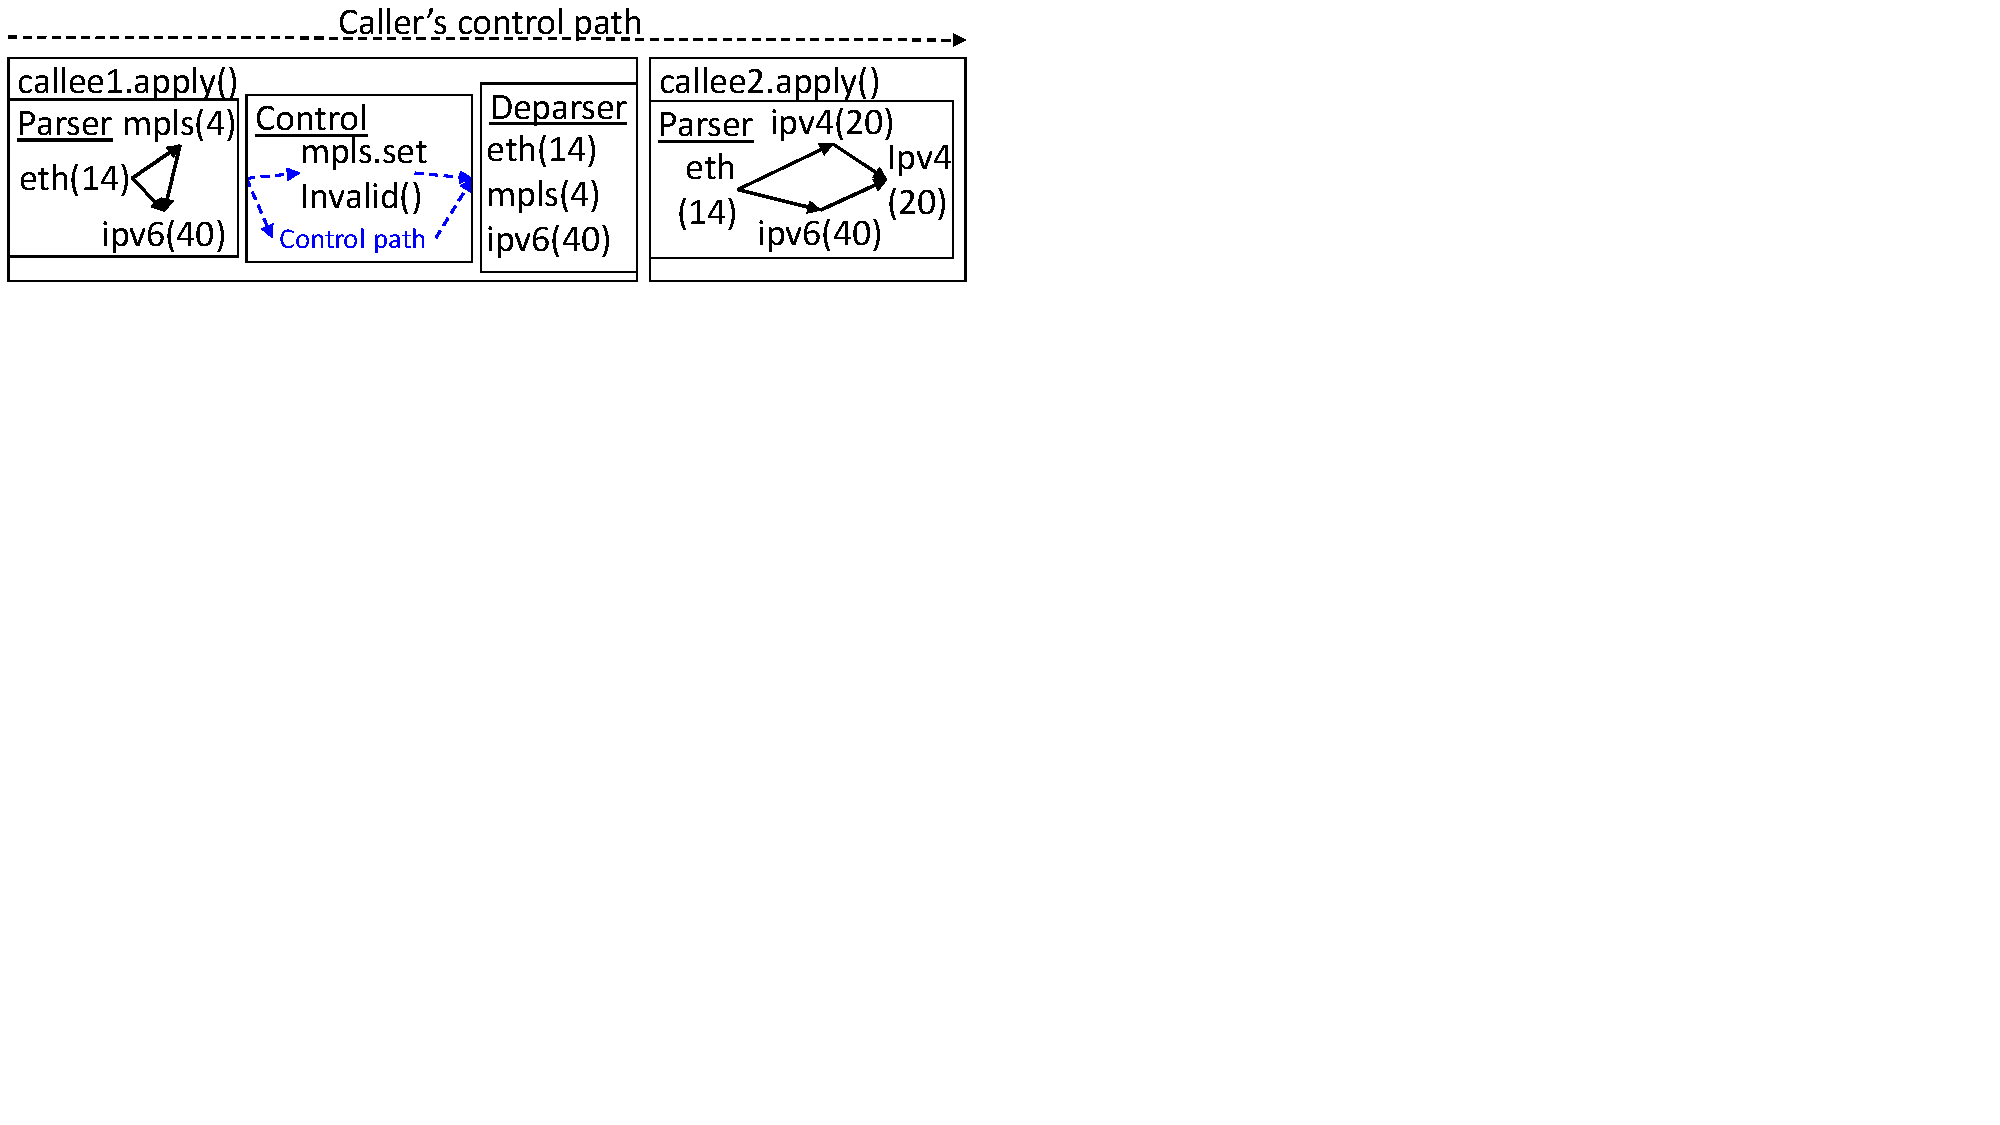
\includegraphics[trim=0 396 487 0, clip,scale=0.5]{sequential-callees}
    \caption{Multiple Callees in a control path}
    \label{fig:sequential-callees}
\end{figure}
Therefore, we take into account extract-length of every callee program's parser along with maximum decrease in packet size by the callee's predecessors in the control path $x$ to compute $lc_{a}(x)$, as shown in (\ref{extract-length-control-path}).
\begin{align}
lc_{a}(x) \; =& \; \max_{p} \left\{ \left( \sum_{i=0}^{i<p} \delta(i) \right)+ \mathcal{E}l(p) \right\},&p \in [0,N] \label{extract-length-control-path} \\
\mathcal{B}s_{a} \; =& \; \mathcal{E}l(a) + \Delta(a) & \label{byte-stack-size-program}
\end{align}
Finally, we define byte-stack size of a program $a$, $\mathcal{B}s_{a}$ (\ref{byte-stack-size-program}), as the sum of its extract-length and maximum increase in packet size.
For the example shown in Figure \ref{fig:sequential-callees}, the byte-stack size of the caller is 98, 20 bytes (due to ipv4.setValid()) in addition of its extract-length.


\subsection{Parser To Match-Action Table}
\label{subsection:parser-to-match-action-table}
\begin{figure*}
    \begin{subfigure}[b]{0.25\linewidth}
        \centering
        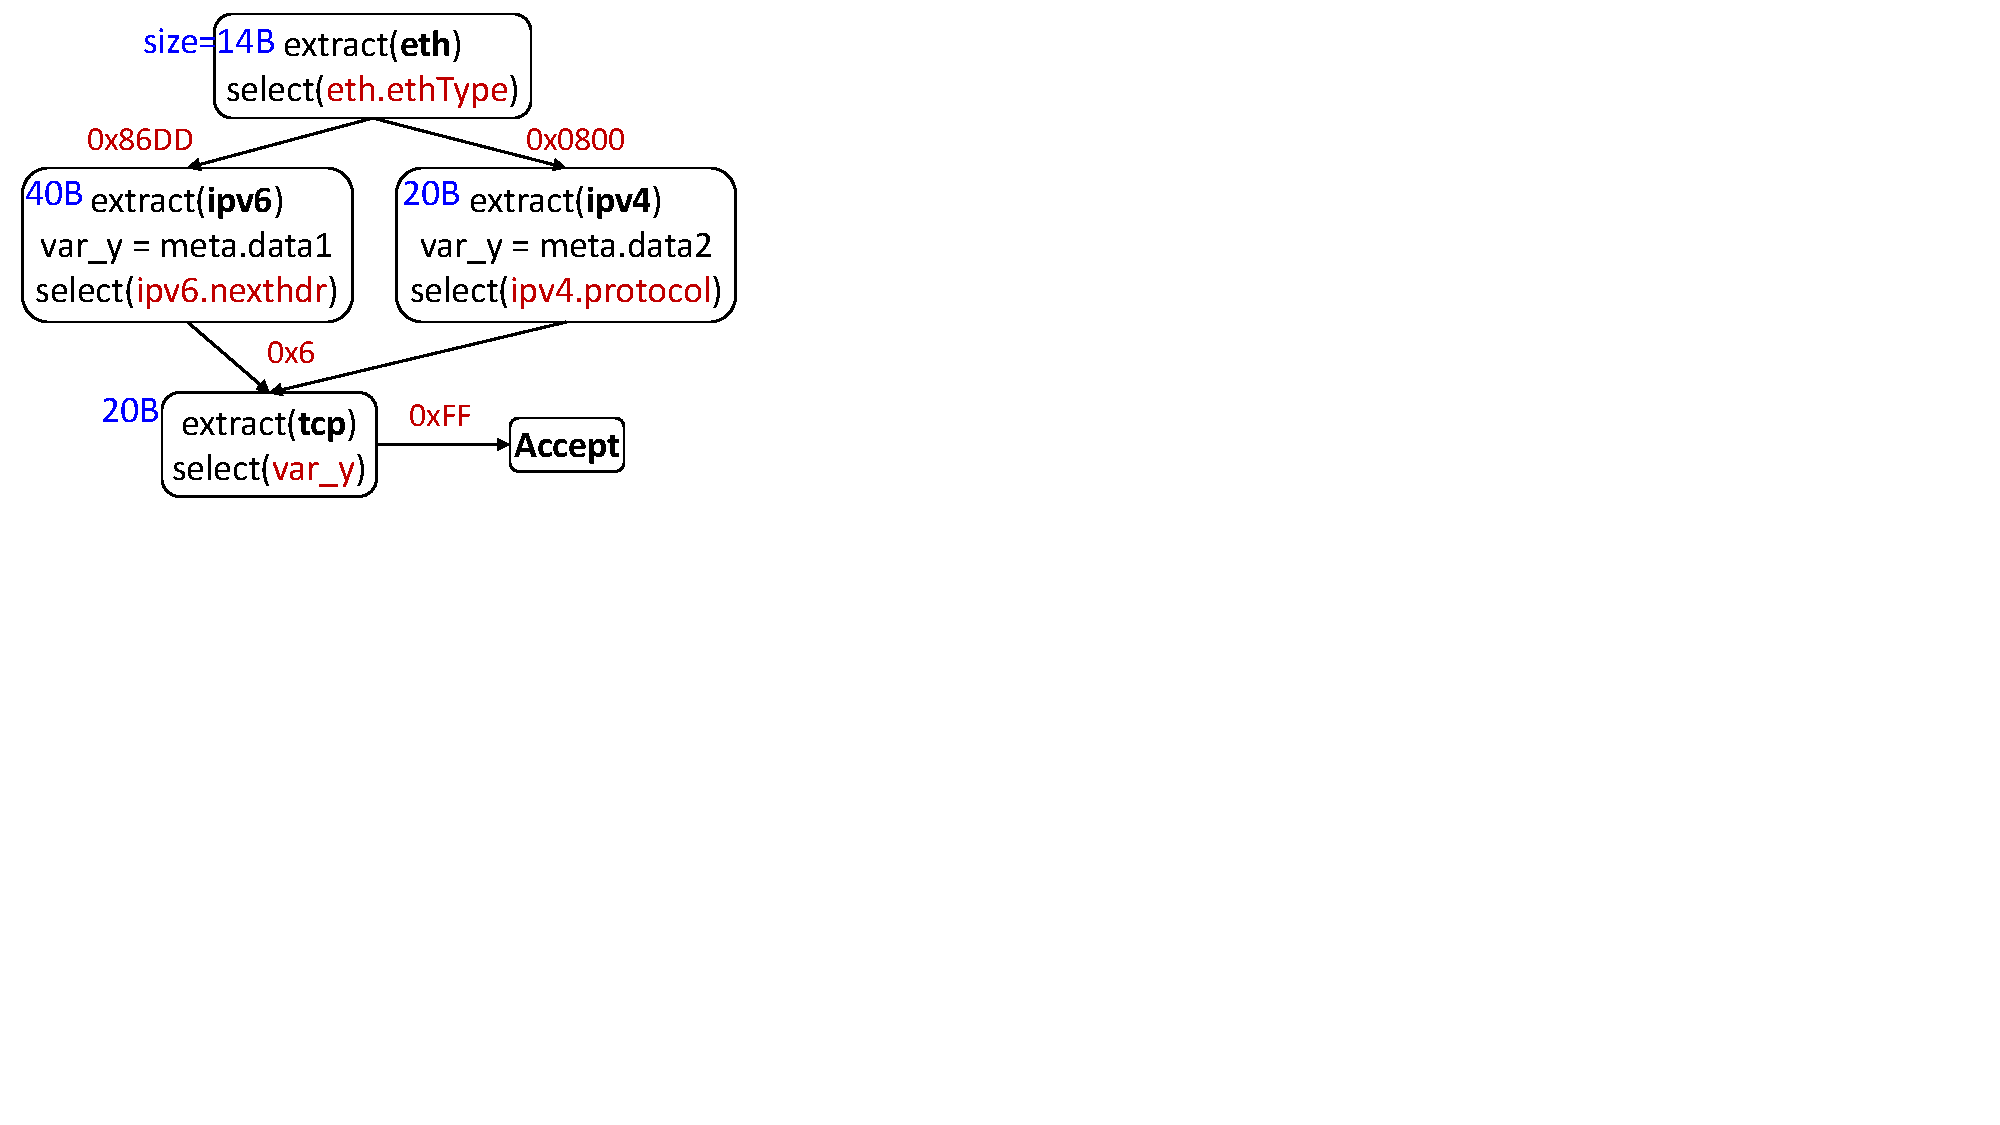
\includegraphics[trim=4 270 596 0, clip,scale=0.37]{parser-transformation-example}    
        \caption{An example P4 Parser}
        \label{subfig:parser}
    \end{subfigure}
    \begin{subfigure}[b]{0.26\linewidth}
        \centering
        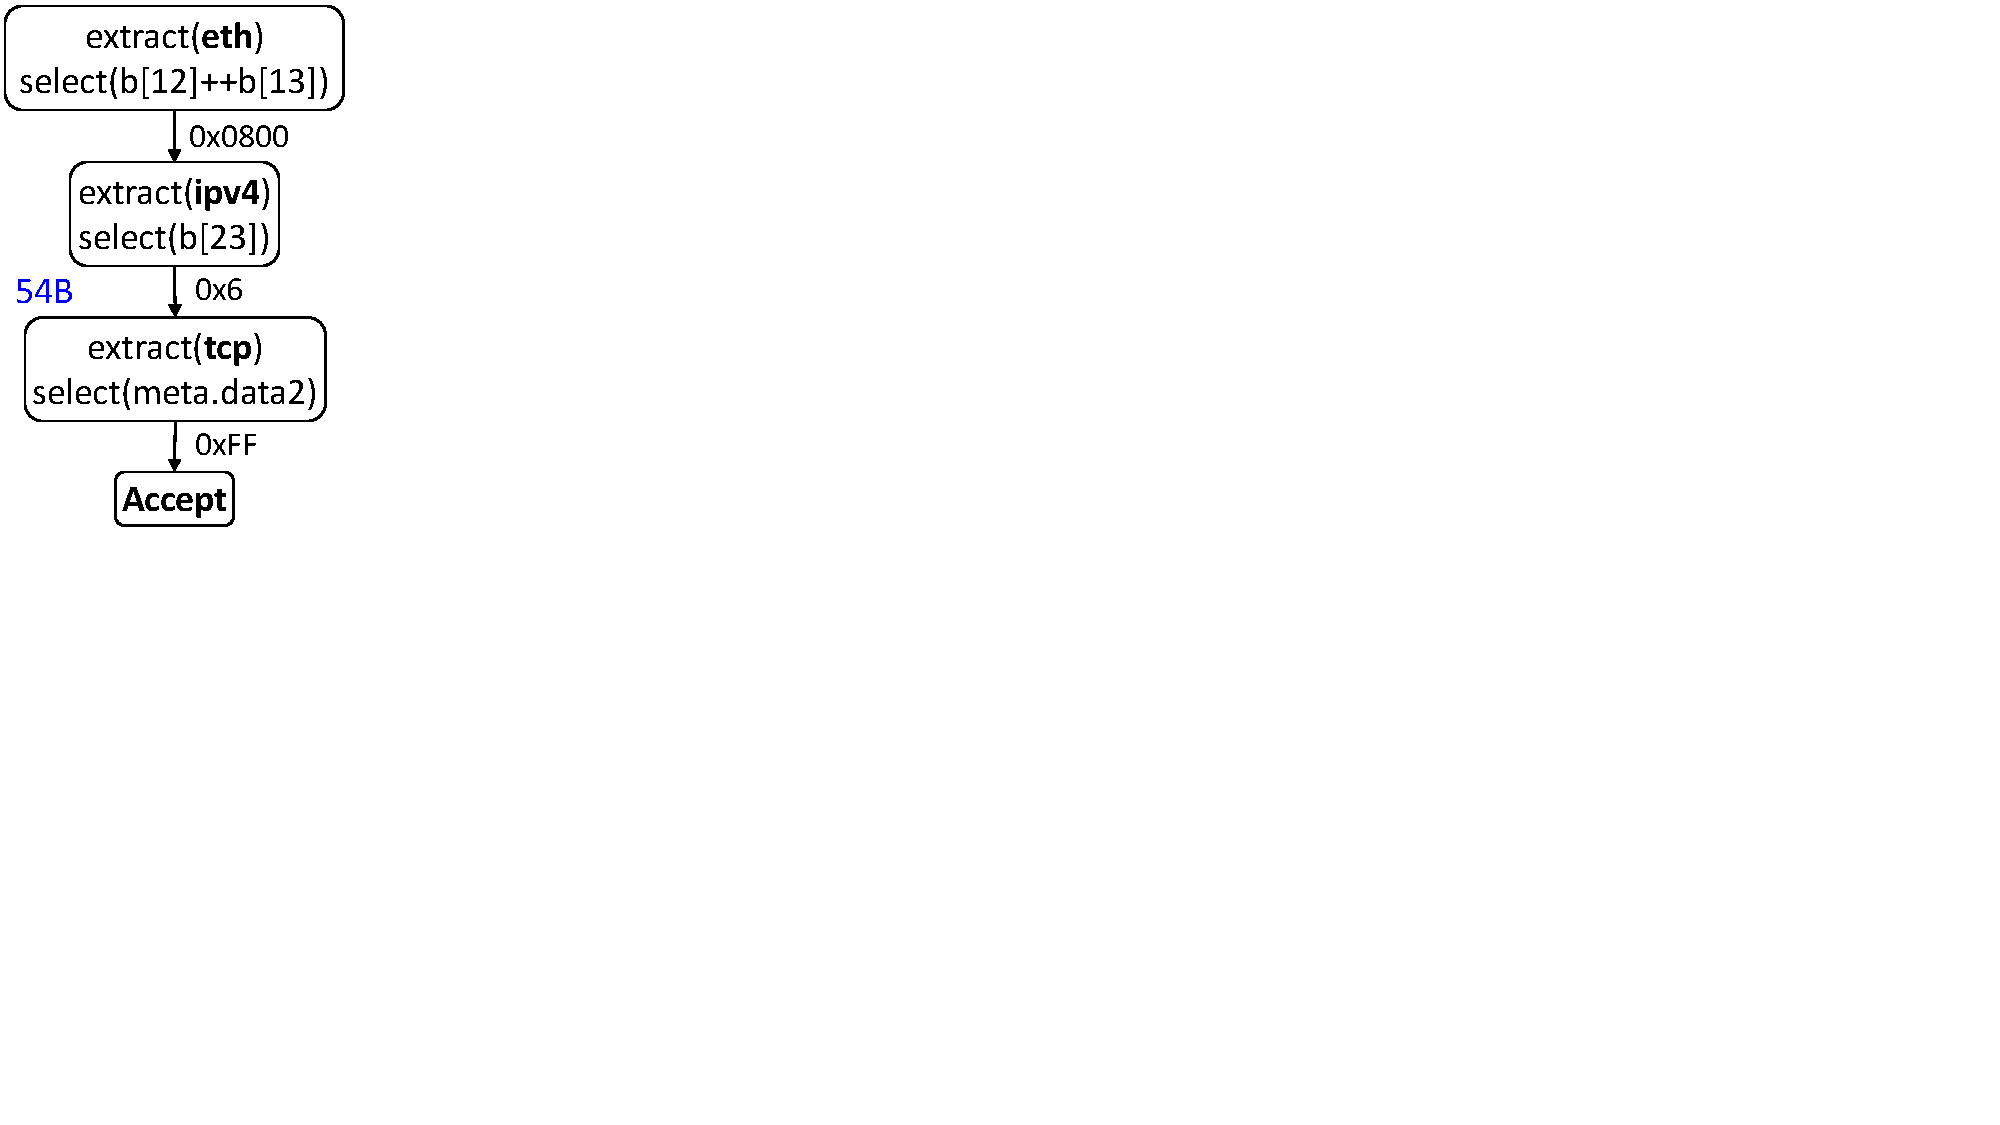
\includegraphics[trim=0 285 794 0, clip,scale=0.37]{parser-example-se-1}
        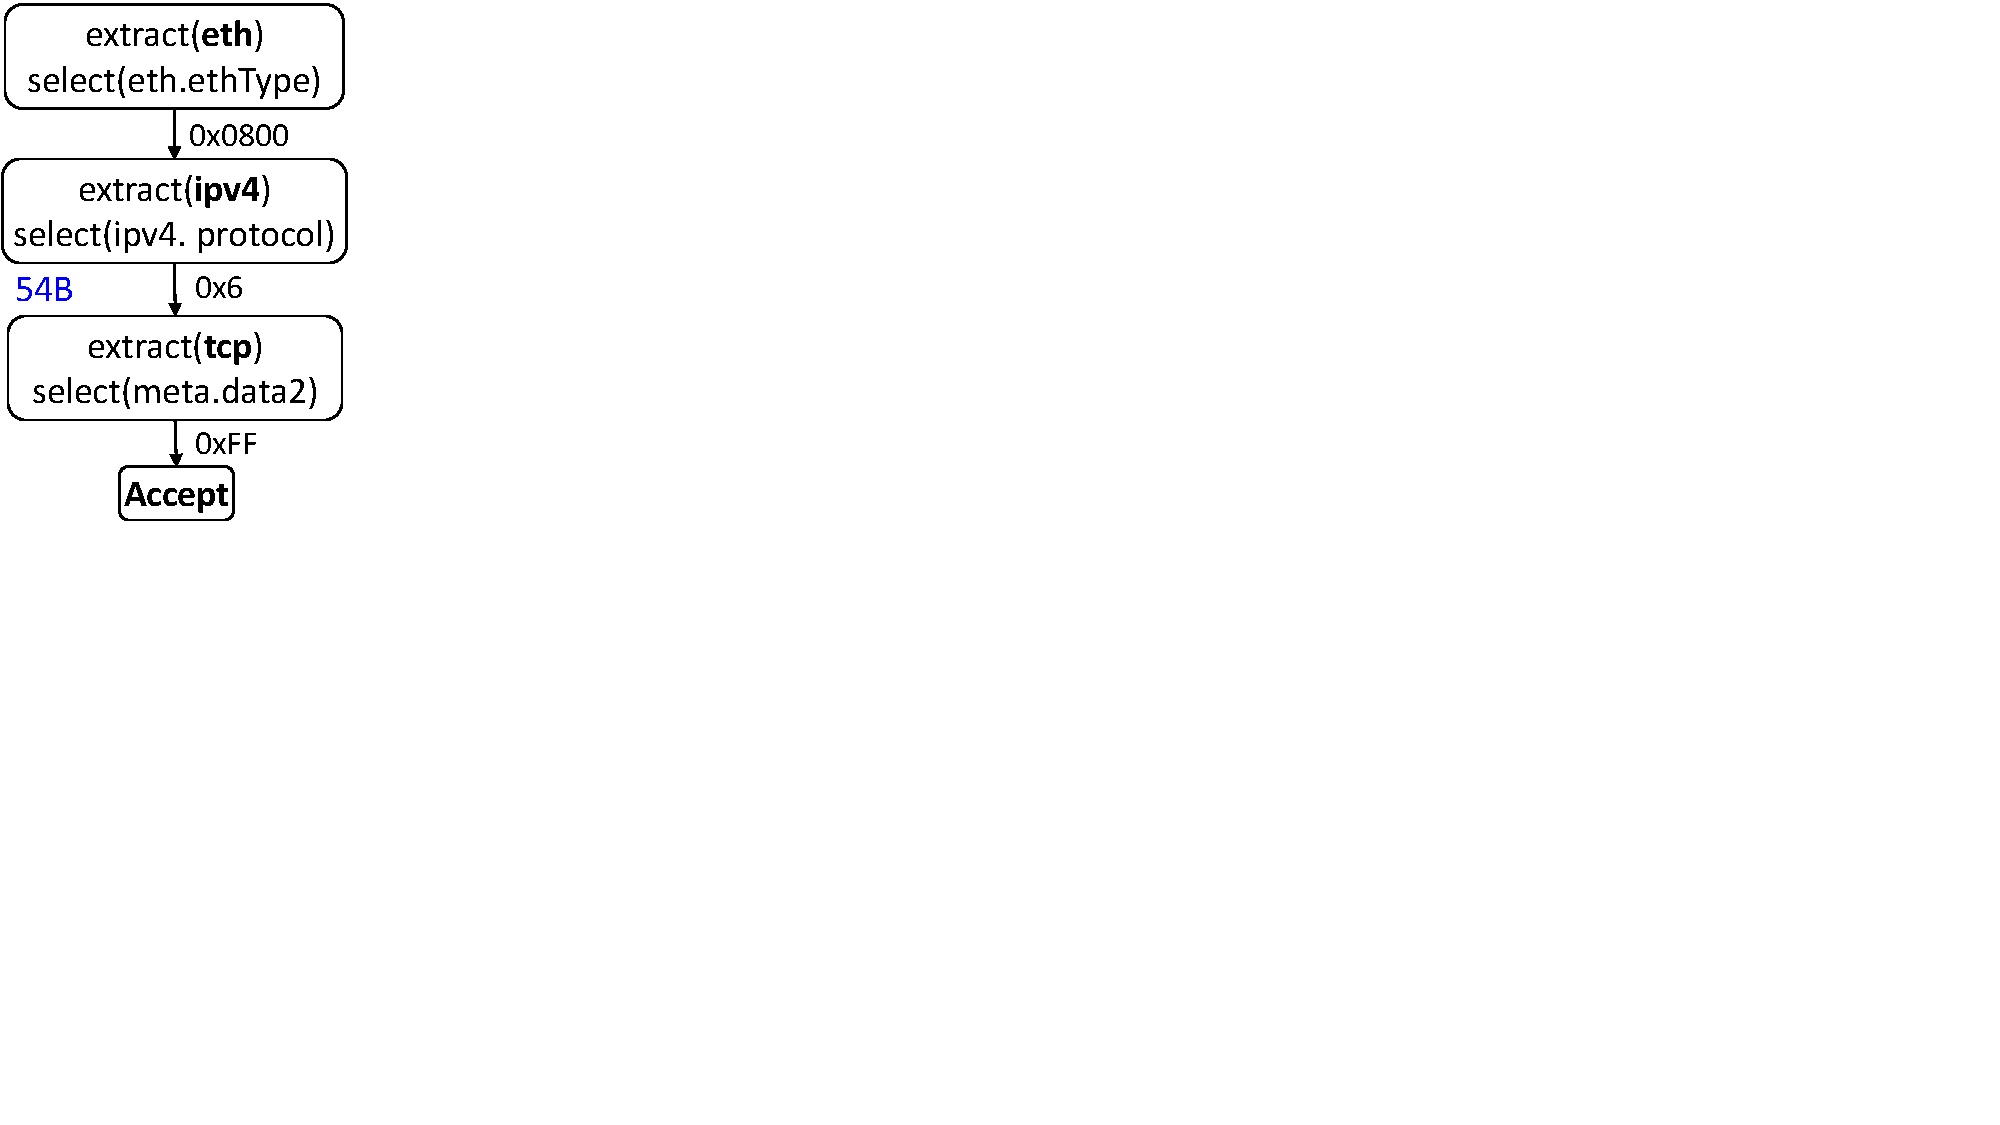
\includegraphics[trim=0 285 794 0, clip,scale=0.37]{parser-example-se-2}
        \caption{Parser Symbolic Execution}
        \label{subfig:parser-symbolic-execution}
    \end{subfigure}
    \begin{subfigure}[b]{.47\linewidth}
    \centering
    \begin{lstlisting}[frame=none]
key = { b[12]++b[13]:exact; // rest Ternary
  b[20]; b[23]; meta.data1; meta.data2;
  b[53].isValid(); b[73].isValid();}
actions = { cp_eth_ipv4_tcp;
  cp_eth_ipv6_tcp; set_parser_error;}
const entries = {
  (x0800,_,x6,_,xFF,1,_):cp_eth_ipv4_tcp();
  (x86DD,x6,_,xFF,_,_,1):cp_eth_ipv6_tcp();
}
default_action : set_parser_error();
\end{lstlisting}
\vspace*{-10pt}
\caption{Match-Action Control Block}
\label{subfig:parser-mat}
\end{subfigure}
\caption{Parser to Control Block Transformation}
\label{fig:parser-to-control-block-transformation}
\end{figure*}

% P4 parser blocks describe parse graphs as state machines.
% Real target devices contain programmable parser module that can be programmed using parse graphs.
% From the design of programmable parser \cite{6665172}, we make following observations.
Programmable parsers \cite{6665172} are implemented as finite state machines using buffer, Ternary Content-Addressable Memories (TCAM) and Action RAM. 
TCAM matches values of current state, fields or variables to identify next state.
Based on the match, headers are copied from byte stream followed by current state update.
Programmable parsers essentially perform repeated match-action operations.
% Network packets are of finite length, hence they can be parsed in a finite number of ways.
Successful parsing of a packet is essentially finding a match for a finite number of bytes from a finite set of values.
Every path enumerated by symbolic execution identifies possible byte locations to match for extracting a set of headers instances.
We leverage match capability of TCAM in match-action stages to match simultaneously all possible byte locations pertaining to every path from start to the accept state.
The action associated with the matched entry copies values from the appropriate locations in the byte-stack to local metadata synthesized for used header fields. 

We describe transformation of parser to match-action control block using the example shown in figure \ref{subfig:parser}.
The parser has four states to extract standard Ethernet, IPv4, IPv6 and TCP headers of size 14, 20, 40 and 20 bytes, respectively.
In general, we consider that parser state may use any metadata or variable to transit to next state. 
As an example, \emph{tcp} state transits to the accept state based on value (0xFF) of \texttt{var\_y} variable which is updated by either \emph{ipv4} or \emph{ipv6} states.
The symbolic execution of the parser computes two possibles paths from the start state to the accept state.
It also computes byte locations for header (e.g., eth.ethType, ipv6.nexthdr, ipv4.protocol) fields used in select expressions of states in the path.
If the select expression depends on local variables, it performs Forward Substitution \cite{Padua:1986:ACO:7902.7904} on every path to eliminate data dependency.
Figure \ref{subfig:parser-symbolic-execution} shows evaluated parser states and two paths generated by symbolic execution with forward substitution.
Every extract method-call statement is transformed into assignments from the byte-stack to field-variables associated with the header instance passed as an argument to the method-call.
In addition, valid metadata variable pertaining to the header instance is set.
We synthesize match-key using union of the select expressions in all the states on every path.
The match-key also comprises valid bit flag of the last byte extracted on every path to consider packet-length in the byte-stack.
For each path, we synthesize an action (e.g., \texttt{cp\_eth\_ipv4\_tcp} in Figure \ref{subfig:parser-mat}) comprising assignment statements in all the states on the path.
We create a match-action entry for every path using case values in select expressions and the action synthesized for the path.
For example, in the first entry shown in Figure \ref{subfig:parser-mat}, x0800, x6, xFF are match-values for the first, third and fifth keys to parse byte-stack as ehternet, ipv4 and tcp headers.
The second and the forth keys can have any values, hence they are matched with don't care values.




% The select expression in transition statement could be a header field, metadata or local variable declared in the parser.
% The value of select expression of a state may depend on its ancestors' parser statements. <<as shown in diagram>>
% Therefore, we perform Forward Substitution on select expressions in evaluated instances of states
% % (https://dl.acm.org/citation.cfm?id=7904)
% on each path and eliminate such data dependency.

% We synthesise local binary variables, called \emph{visit},  for each parser state to track the state transition of the parser's FSM.
% For every evaluated instance of a parser state, we synthesise an action comprising its parser\-Statements and replace extract method call statements to assignment statements.
% The assignment statements copies bytes from the buffer array to header instances' fields according to their sizes.
% Next, we add pop method call with the header size as the argument to remove the header from the byte array.
% We insert setValid method call statement for the extracted header instances.
% We add an assignment statement to set visit variable associated with the parser state.

\subsection{Transformation To Simple Parser}
% \subsection{Header Stacks \& Variable-Length Headers}
\label{subsection:header-stacks-variable-length-headers}
$\mu$P4 allows to use of header stacks with their size known at compile-time. 
$\mu$P4C replaces every header stack instance with multiple instances of the header type. 
It symbolically evaluates operations on the header stack instances and transforms them into appropriate built-in method calls of the instances.
P4 provides various sets of computations to use in parser and control blocks.
In parser blocks, programmers can use \texttt{next} and \texttt{last} operations to iterate through the stack.
These operations along with \texttt{lastIndex} can be used to write loops in parsers to extract instances in header stack.
$\mu$P4C unrolls such loops by replicating the parse states in them.
Loop unrolling replaces relative referencing operations, \texttt{next} and \texttt{last}, with appropriate header instances in the state replicas.
P4 provides \texttt{push\_front} and \texttt{pop\_front} operations on stack instances to manipulate elements on top and bottom of the stack.
$\mu$P4C transforms push\_front and pop\_front operations into series of assignments and built-in method calls of header instances.
For example, assume that \texttt{hs} is a header stack instance of size 3. 
$\mu$P4C synthesize hs0, hs1, hs2 header instances to replace hs.
\texttt{hs\_inst.push\_front(1)} is replaced with \texttt{hs2 = hs1}, \texttt{hs1 = hs0} and \texttt{hs0.setInvalid()}.


$\mu$P4 allows programmers to define variable-length header types, however it imposes a constraint that their variable-length fields must contain integer number of bytes at runtime.
% $\mu$P4C splits header type containing fixed and variable-length fields into multiple types, where each type contains either fixed-length fields or the variable-length field.
$\mu$P4C transforms every parser state with two-argument extract method call, used to extract variable-length header, into a sub-parser.
It splits the header type of the instance in the first argument into multiple types, where each type contains either fixed-length fields or the variable-length field.
Every state in the sub-parser extracts a fixed-number of bytes from the packet bit stream.
The sub-parser contains a state having the second argument (variableFieldSize) as the expression in its select statement.
The select statement has case-list enumerating all possible values up to specified maximum size of the variable-length field.
For each select case, the sub-parser transits to a state extracting a fixed number of bytes in the variable-length field.
For example, if variable-length field has maximum size of 40 bytes, $\mu$P4C creates 40 states extracting different number of bytes.
The explosion of number of states would only increase number of entries in the transformed match-action table of the parser.

% \begin{figure}[H]
% \begin{minipage}[c]{0.45\linewidth}
% \begin{lstlisting}[frame=none]
% header_t[3] hs;
% 
% hs.push_front(1);
% \end{lstlisting}
% \end{minipage}
% \begin{minipage}[c]{0.45\linewidth}
% \begin{lstlisting}[frame=none]
% header_t hs0, hs1, hs2;
% 
% hs2 = hs1;
% hs1 = hs0;
% hs0.setInvalid()
% \end{lstlisting}
% \end{minipage}
% \caption{Extern to }
% \label{fig:}
% \end{figure}



\subsection{Deparser To Match-Action Table:}
\label{subsection:deparser-to-match-action-table}
The deparser blocks of $\mu$SA's pipelines are the control blocks with emitter as one of the parameters.
$\mu$P4C replaces the emitter instance's emit method-call statements with match-action table to transform deparser into normal match-action control blocks.
The match-action table copies back field-variables to appropriate locations in byte-stack based on values of valid metadata variables associated with header instances. 
The control block of the pipeline may set or reset validity of header instances and, thereby, modifying the size of the packet.
In case of increase in packet size, byte-stack is always large enough to hold new headers.
If a deparser decreases the packet size, subsequent parsers may set \texttt{packet\_too\_short} error only if packet-length on the wire is less than the extract-length and greater than the min-packet-size for the main program.

The symbolic execution of a deparser derives the emit order of header instances in the block.
Using the size of header instances and the emit order, we compute offsets in byte-stack to copy back field-variables and to insert new header fields.
The match key comprises valid metadata variables associated with each header instance in the program.
For every possible combination of valid headers, we synthesize a series of operations on byte-stack as an action to copy field-variables and to move data in byte-stack.
The control block of callee1 shown in Figure \ref{fig:sequential-callees} invalidates the mpls header from packets if the execution follows a particular control path.
Recall that, the parser synthesized by $\mu$P4C extracts 78 bytes in the stack.
If the execution follows control path invalidating mpls header, 60 bytes following the header should be moved up by the offset of 4 in the stack.
The synthesized action performs in-place copy of these 60 bytes. It invalidates the last 4 bytes.
If the control block execution sets ipv4 header instance to valid, bytes after the ipv6 header are pushed down by the offset of 20 to insert ipv4 header instance.



\subsection{Real-Target Specific Transformation}
$\mu$P4C transforms the programs described using $\mu$P4's data plane abstractions into a given real target specific ones.
$\mu$SA defines logical pipelines and externs to provide abstraction for data plane pipelines.
As a part of data plane abstractions, $\mu$SA allows to describe multiple packet processing in control blocks of its orchestration pipelines.
Programmers can create multiple copies of packets in the control blocks using \texttt{copy\_from} methods of $\mu$SA externs to describe multi-packet processing.
$\mu$P4C's transformations create copies of packet using externs provided by the architecture of the specified target.
$\mu$P4C realizes multi-packet processing by identifying a packet-processing sub-graph, called a \emph{thread}, for every definition of a \texttt{pkt} instance.
% Existing target devices can not process multiple packets by the same thread at the same time.
Then, it prepares \emph{Packet-Processing Schedule} (PPS) of the threads in the program and maps it to packet-processing blocks of the target's architecture.
Some target architectures may impose constraint that PPSs must be serializable.
If $\mu$P4C fails to find a serial PPS for such targets, it raises a compilation error. 


\subsubsection{Packet-Processing Schedule}
$\mu$P4C extracts packet-processing threads from the control block of orchestration pipeline's interface while maintaining control and data dependencies.
To this end, it constructs a Program Dependence Graph(PDG) \cite{Ferrante:1987:PDG:24039.24041} and performs a series of transformations.

$\mu$P4C treats parameter of orchestration control block or every \texttt{copy\_from} method call statement of \texttt{pkt} instance as its definition, because they initialize the instance.
We note that \texttt{pkt} instance argument in \texttt{copy\_from} method calls is only used or read.
Moreover, all other method call statements having \texttt{pkt} instances as arguments access (read and modify) the instances, such call statements are not considered as their definition statements.


We define \emph{access ranges} of a \texttt{pkt} instance's definition as span of program statements until the next definition of the instance in reached on every possible path in the PFG.
We merge overlapping access ranges of multiple definitions of the same \texttt{pkt} instance.
Non overlapping access ranges of the same instance are renamed to create one-to-one mapping between an instance and its access range.
Inspired from \emph{program slice} defined in \cite{Weiser:1981:PS:800078.802557}, we define \emph{packet slice} based on access ranges of \texttt{pkt} instances' definitions.
A packet slice of a \texttt{pkt} instance is an executable subset of PDG, which consists of all the program statements affecting the instance's value in overlapping access ranges of its definitions.
Packet slices can have multiple entry and exist points.
A set of definition statements of \emph{pkt} instance with overlapping access ranges is considered as a slicing criteria for a given packet instance.
We compute packet slices from the PDG of control block using a method similar to one described in \cite{Ferrante:1987:PDG:24039.24041}.
Specifically, we perform a graph traversal in reverse direction of edges from every statement at exit points in the access ranges until definition statements in the criteria set are reached.
The graph traversal continues until all possible definitions of every variable used in visited statement are reached.
If any variable or extern instance is involved in anti-dependency, it is resolved by introducing new variable and renaming.
An example program shown in Figure \ref{fig:multi-packet-processing} is sliced with respect to definitions of three instances \texttt{pm}, \texttt{p} and \texttt{pt}.


Packet slices of different instances may have common program statements due to control and data dependence.
Therefore, a packet slice may have method call statements processing different \emph{pkt} instances than one's definition statements used in slicing criteria.
For the program shown in Figure \ref{fig:multi-packet-processing}, slice 1 pertaining to instance \texttt{pm} shares program statements with slices 2 and 3 related to \texttt{p} and \texttt{pt}, respectively.
We create a packet-processing thread per instance by excluding such method call statements from every packet slice but maintain dependence among them by creating inter-thread dependence.
All the common program statements not accessing \texttt{pkt} instances are also excluded from threads.
We term such statements \emph{cps} nodes and maintain their control and data dependencies with the thread nodes.
We associate every thread with an identifier, \emph{thread-id}, and a set of group-ids, called \emph{clone-group}.
Every thread-id identifies a thread based on unique \texttt{pkt} instance processed by it.
Every group-id identifies set of threads that may process copies of the same packet instance.
In presence, of conditional statements like if-else and switch, a thread may process a copy of a packet from multiple possible clone groups.

% and clone-group identifies every possible \texttt{pkt} instances from which the thread's packet instance could be initialized.


We transform PDG to PPS graph by coalescing all the nodes in a thread to a single node while maintaining their control and data dependencies with cps and other thread nodes.
We synthesise a variable to transform every control dependency among thread nodes to a data dependency.
The thread, which is depended on, sets the variable with a constant value and the other thread uses the variable in predicate of new if-conditional statement to continue processing on the control path.
If a PPS has a directed cycle involving thread nodes, PPS is not serializable.
If the real target does not have capability to process multiple copy of a packet at the same time, 
$\mu$P4C raises error and lists program statements involved in cycles.
However, a PPS can have cycles involving maximum one thread node and common program statements represented by cps nodes.
To decide execution thread for cps nodes, we compute strongly connected components of PPS graph.
In each component, there can be exactly one thread node and one or more cps nodes.
We further transform PPS into a directed acyclic graph by contracting each component into a single node.
PPS can still have cps nodes not part of any strongly connected component, such nodes can be executed as a part of any thread with which they have dependence.
We schedule such cps nodes while mapping the thread nodes to packet-processing blocks of target architecture.



% Every \texttt{apply} method call statement of \texttt{Multicast} or \texttt{Orchestration} type package gets transformed to a thread node in PPS.
% \texttt{enqueue}, \texttt{merge} and \texttt{to\_in\_buf} method call statements of \texttt{out\_buf} extern's instances capture dependence among such threads nodes in PPS.



\subsubsection{Mapping to Target Architecture}
$\mu$P4C visits PPS nodes in topological order to map thread and cps nodes on target architecture.
Also, standard metadata (\texttt{sm\_t}) instances and logical extern instances (\texttt{es\_t} and \texttt{mc\_engine}) used in the program are translated into intrinsic metadata and extern provided by the target architecture.
$\mu$P4C partitions the sub-program represented by each thread node in multiple packet-processing block according to pipeline model of the target architecture.


Let's consider v1model architecture of simple\_switch target device for an example.
We create a two-state, named ingress and egress, finite-state machine to capture restriction on usage of egress-spec, egress-port and queuing metadata in ingress and egress blocks.
Each state represents a set of assertions to be verified on program statements while visiting them in topological order.
State transition occurs when the graph traversal can not be continued due to absence of nodes without incoming edges.
In the ingress state, the graph traversal asserts that every visited statement is not $1$ a call of apply method of \texttt{mc\_engine}  and $2$ \texttt{get\_value method} methods of \texttt{egress\_spec}.
When the traversal can not progress any further state transition happens and we split the thread PDG into two PDGs of visited and non-visited nodes.
In the egress state, the graph traversal asserts every that visited statement is not a method call of \texttt{get\_egress\_port}.

There can be multiple edges representing control branches between the partitions.
We synthesize \emph{partition} metadata that is assigned a unique value for each control branch in the first partition.
The second partition uses the metadata and condition on their values to resume execution on appropriate control branch.
Also, partitioned code may access the same local declaration variables.
These shared local variables along with the \emph{partition} metadata are passed as user-defined metadata between ingress and egress control block.

We synthesize per packet user metadata to store thread-id.
A packet is processed by a thread only if the corresponding thread-id is set in the metadata. 
We enforce this condition by instrumenting thread code with an if-conditional statement.
At the end of each thread, next thread-id is set.





%-------------------------------------------------------------------------------
\section*{Acknowledgments}
%-------------------------------------------------------------------------------

The USENIX latex style is old and very tired, which is why
there's no \textbackslash{}acks command for you to use when
acknowledging. Sorry.

%-------------------------------------------------------------------------------
\section*{Availability}
%-------------------------------------------------------------------------------

USENIX program committees give extra points to submissions that are
backed by artifacts that are publicly available. If you made your code
or data available, it's worth mentioning this fact in a dedicated
section.

%-------------------------------------------------------------------------------
\bibliographystyle{plain}
\bibliography{main}


\appendix
\section{Micro Switch Architecture}
\begin{figure}
\begin{lstlisting}[frame=none]
extern pkt {
  // byte array representation
  byte[] packet;
  unsigned length;
  void copy_from(pkt p);
}
extern emitter {
  void emit<H>(pkt p, in H hdr);
}
extern extractor {
  void extract<H>(pkt p, out H hdr);
  void extract<H>(pkt p, out H hdr, in bit<32> size);
  /// H may be an arbitrary fixed-size type.
  H lookahead<H>();
}
\end{lstlisting}
\caption{Packet Representation}
\label{fig:pkt-externs}
\end{figure}
\begin{figure}

\begin{lstlisting}[frame=none]
enum meta_t {
  INGRESS_TIMESTAMP,
  EGRESS_TIMESTAMP
}
extern es_t {
  void set_out_port(in bit<8>);
  bit<8> get_out_port();
  bit<32> get_value(in meta_t ft);
  void copy_from(es_t es);
}
\end{lstlisting}
\caption{\texttt{es\_t} extern}
\label{fig:msa-egress-spec-extern}
\end{figure}
\begin{figure}
\begin{lstlisting}[frame=none]
extern in_buf<I> {
  // used by architecture only
  dequeue(pkt, out sm_t, es_t, out I);
}
extern out_buf<O> {
  enqueue(pkt p, in sm_t sm, es_t es, in O out_args);
  void to_in_buf(in_buf<O>);
  void merge(out_buf<O>);
}

extern mc_buf<H, O> {
  enqueue(pkt, in H, in sm_t, es_t, in O);
  dequeue(pkt, out H, out sm_t, es_t, out O);
}
\end{lstlisting}
\caption{Buffer Representation}
\label{fig:pkt-buf}
\end{figure}

\begin{figure}
\begin{lstlisting}[frame=none]
// This can only be used in control block of multicast interface
extern mc_engine {
  mc_engine();
  void set_mc_group(GroupId_t gid);
  apply(es_t, out PacketInstanceId_t);
  
  set_buf(out_buf<O>);
  apply(pkt, out sm_t, es_t, out O);  
}
\end{lstlisting}
\caption{Multicast Extern}
\label{fig:msa-multicast-extern}
\end{figure}


\begin{figure}
\begin{lstlisting}[frame=none]
// Unicast
Unicast<H,M,I,O,IO>(pkt p, inout sm_t sm, es_t es, in I in_param, out O out_param, inout IO inout_param) {
  parser u_parser(extractor ex, pkt p, out H hdr, inout M meta, inout sm_t sm, in I in_param, inout IO inout_param);
  control u_control(pkt p, inout H hdr, inout M m, inout sm_t sm, es_t es, in I in_param, out O out_param, inout IO inout_param);
  control u_deparser(emitter em, pkt p, in H hdr);                             
}

// Multicast
Multicast<H,M,I,O>(pkt p, in sm_t sm, es_t es, in I in_param, out_buf<O> ob) {
  parser m_parser(extractor ex, pkt p, out H hdr, inout M meta, in I in_param, inout sm_t sm);
  control m_control(pkt p, inout H hdr, inout M meta, inout sm_t sm, es_t es, inout I in_param, mc_buf<H,O> mob);
  control m_deparser(emitter em, pkt p, in H hdr);
}

package Orchestration<I,O>(in_buf<I> ib, out_buf<O> ob) {                         
  control o_control(pkt p, inout sm_t sm, es_t es, in I in_param, out_buf<O> ob);
}
    
\end{lstlisting}
\caption{Programmable Blocks for Interfaces}
\label{fig:programmable-blocks-for-interfaces}
\end{figure}

%%%%%%%%%%%%%%%%%%%%%%%%%%%%%%%%%%%%%%%%%%%%%%%%%%%%%%%%%%%%%%%%%%%%%%%%%%%%%%%%
\end{document}
%%%%%%%%%%%%%%%%%%%%%%%%%%%%%%%%%%%%%%%%%%%%%%%%%%%%%%%%%%%%%%%%%%%%%%%%%%%%%%%%

%%  LocalWords:  endnotes includegraphics fread ptr nobj noindent
%%  LocalWords:  pdflatex acks
